% Options for packages loaded elsewhere
% Options for packages loaded elsewhere
\PassOptionsToPackage{unicode}{hyperref}
\PassOptionsToPackage{hyphens}{url}
\PassOptionsToPackage{dvipsnames,svgnames,x11names}{xcolor}
%
\documentclass[
  chinese,
]{ctexart}
\usepackage{xcolor}
\usepackage[margin=1in]{geometry}
\usepackage{amsmath,amssymb}
\setcounter{secnumdepth}{-\maxdimen} % remove section numbering
\usepackage{iftex}
\ifPDFTeX
  \usepackage[T1]{fontenc}
  \usepackage[utf8]{inputenc}
  \usepackage{textcomp} % provide euro and other symbols
\else % if luatex or xetex
  \usepackage{unicode-math} % this also loads fontspec
  \defaultfontfeatures{Scale=MatchLowercase}
  \defaultfontfeatures[\rmfamily]{Ligatures=TeX,Scale=1}
\fi
\usepackage{lmodern}
\ifPDFTeX\else
  % xetex/luatex font selection
\fi
% Use upquote if available, for straight quotes in verbatim environments
\IfFileExists{upquote.sty}{\usepackage{upquote}}{}
\IfFileExists{microtype.sty}{% use microtype if available
  \usepackage[]{microtype}
  \UseMicrotypeSet[protrusion]{basicmath} % disable protrusion for tt fonts
}{}
\makeatletter
\@ifundefined{KOMAClassName}{% if non-KOMA class
  \IfFileExists{parskip.sty}{%
    \usepackage{parskip}
  }{% else
    \setlength{\parindent}{0pt}
    \setlength{\parskip}{6pt plus 2pt minus 1pt}}
}{% if KOMA class
  \KOMAoptions{parskip=half}}
\makeatother
% Make \paragraph and \subparagraph free-standing
\makeatletter
\ifx\paragraph\undefined\else
  \let\oldparagraph\paragraph
  \renewcommand{\paragraph}{
    \@ifstar
      \xxxParagraphStar
      \xxxParagraphNoStar
  }
  \newcommand{\xxxParagraphStar}[1]{\oldparagraph*{#1}\mbox{}}
  \newcommand{\xxxParagraphNoStar}[1]{\oldparagraph{#1}\mbox{}}
\fi
\ifx\subparagraph\undefined\else
  \let\oldsubparagraph\subparagraph
  \renewcommand{\subparagraph}{
    \@ifstar
      \xxxSubParagraphStar
      \xxxSubParagraphNoStar
  }
  \newcommand{\xxxSubParagraphStar}[1]{\oldsubparagraph*{#1}\mbox{}}
  \newcommand{\xxxSubParagraphNoStar}[1]{\oldsubparagraph{#1}\mbox{}}
\fi
\makeatother

\usepackage{color}
\usepackage{fancyvrb}
\newcommand{\VerbBar}{|}
\newcommand{\VERB}{\Verb[commandchars=\\\{\}]}
\DefineVerbatimEnvironment{Highlighting}{Verbatim}{commandchars=\\\{\}}
% Add ',fontsize=\small' for more characters per line
\usepackage{framed}
\definecolor{shadecolor}{RGB}{241,243,245}
\newenvironment{Shaded}{\begin{snugshade}}{\end{snugshade}}
\newcommand{\AlertTok}[1]{\textcolor[rgb]{0.68,0.00,0.00}{#1}}
\newcommand{\AnnotationTok}[1]{\textcolor[rgb]{0.37,0.37,0.37}{#1}}
\newcommand{\AttributeTok}[1]{\textcolor[rgb]{0.40,0.45,0.13}{#1}}
\newcommand{\BaseNTok}[1]{\textcolor[rgb]{0.68,0.00,0.00}{#1}}
\newcommand{\BuiltInTok}[1]{\textcolor[rgb]{0.00,0.23,0.31}{#1}}
\newcommand{\CharTok}[1]{\textcolor[rgb]{0.13,0.47,0.30}{#1}}
\newcommand{\CommentTok}[1]{\textcolor[rgb]{0.37,0.37,0.37}{#1}}
\newcommand{\CommentVarTok}[1]{\textcolor[rgb]{0.37,0.37,0.37}{\textit{#1}}}
\newcommand{\ConstantTok}[1]{\textcolor[rgb]{0.56,0.35,0.01}{#1}}
\newcommand{\ControlFlowTok}[1]{\textcolor[rgb]{0.00,0.23,0.31}{\textbf{#1}}}
\newcommand{\DataTypeTok}[1]{\textcolor[rgb]{0.68,0.00,0.00}{#1}}
\newcommand{\DecValTok}[1]{\textcolor[rgb]{0.68,0.00,0.00}{#1}}
\newcommand{\DocumentationTok}[1]{\textcolor[rgb]{0.37,0.37,0.37}{\textit{#1}}}
\newcommand{\ErrorTok}[1]{\textcolor[rgb]{0.68,0.00,0.00}{#1}}
\newcommand{\ExtensionTok}[1]{\textcolor[rgb]{0.00,0.23,0.31}{#1}}
\newcommand{\FloatTok}[1]{\textcolor[rgb]{0.68,0.00,0.00}{#1}}
\newcommand{\FunctionTok}[1]{\textcolor[rgb]{0.28,0.35,0.67}{#1}}
\newcommand{\ImportTok}[1]{\textcolor[rgb]{0.00,0.46,0.62}{#1}}
\newcommand{\InformationTok}[1]{\textcolor[rgb]{0.37,0.37,0.37}{#1}}
\newcommand{\KeywordTok}[1]{\textcolor[rgb]{0.00,0.23,0.31}{\textbf{#1}}}
\newcommand{\NormalTok}[1]{\textcolor[rgb]{0.00,0.23,0.31}{#1}}
\newcommand{\OperatorTok}[1]{\textcolor[rgb]{0.37,0.37,0.37}{#1}}
\newcommand{\OtherTok}[1]{\textcolor[rgb]{0.00,0.23,0.31}{#1}}
\newcommand{\PreprocessorTok}[1]{\textcolor[rgb]{0.68,0.00,0.00}{#1}}
\newcommand{\RegionMarkerTok}[1]{\textcolor[rgb]{0.00,0.23,0.31}{#1}}
\newcommand{\SpecialCharTok}[1]{\textcolor[rgb]{0.37,0.37,0.37}{#1}}
\newcommand{\SpecialStringTok}[1]{\textcolor[rgb]{0.13,0.47,0.30}{#1}}
\newcommand{\StringTok}[1]{\textcolor[rgb]{0.13,0.47,0.30}{#1}}
\newcommand{\VariableTok}[1]{\textcolor[rgb]{0.07,0.07,0.07}{#1}}
\newcommand{\VerbatimStringTok}[1]{\textcolor[rgb]{0.13,0.47,0.30}{#1}}
\newcommand{\WarningTok}[1]{\textcolor[rgb]{0.37,0.37,0.37}{\textit{#1}}}

\usepackage{longtable,booktabs,array}
\newcounter{none} % for unnumbered tables
\usepackage{calc} % for calculating minipage widths
% Correct order of tables after \paragraph or \subparagraph
\usepackage{etoolbox}
\makeatletter
\patchcmd\longtable{\par}{\if@noskipsec\mbox{}\fi\par}{}{}
\makeatother
% Allow footnotes in longtable head/foot
\IfFileExists{footnotehyper.sty}{\usepackage{footnotehyper}}{\usepackage{footnote}}
\makesavenoteenv{longtable}
\usepackage{graphicx}
\makeatletter
\newsavebox\pandoc@box
\newcommand*\pandocbounded[1]{% scales image to fit in text height/width
  \sbox\pandoc@box{#1}%
  \Gscale@div\@tempa{\textheight}{\dimexpr\ht\pandoc@box+\dp\pandoc@box\relax}%
  \Gscale@div\@tempb{\linewidth}{\wd\pandoc@box}%
  \ifdim\@tempb\p@<\@tempa\p@\let\@tempa\@tempb\fi% select the smaller of both
  \ifdim\@tempa\p@<\p@\scalebox{\@tempa}{\usebox\pandoc@box}%
  \else\usebox{\pandoc@box}%
  \fi%
}
% Set default figure placement to htbp
\def\fps@figure{htbp}
\makeatother



\ifLuaTeX
\usepackage[bidi=basic,shorthands=off,provide=*]{babel}
\else
\usepackage[bidi=default,shorthands=off,provide=*]{babel}
\fi
\ifLuaTeX
  \usepackage{selnolig} % disable illegal ligatures
\fi


\setlength{\emergencystretch}{3em} % prevent overfull lines

\providecommand{\tightlist}{%
  \setlength{\itemsep}{0pt}\setlength{\parskip}{0pt}}



 


\usepackage{bm}
\usepackage{amssymb}
\makeatletter
\@ifpackageloaded{caption}{}{\usepackage{caption}}
\AtBeginDocument{%
\ifdefined\contentsname
  \renewcommand*\contentsname{目录}
\else
  \newcommand\contentsname{目录}
\fi
\ifdefined\listfigurename
  \renewcommand*\listfigurename{图索引}
\else
  \newcommand\listfigurename{图索引}
\fi
\ifdefined\listtablename
  \renewcommand*\listtablename{表索引}
\else
  \newcommand\listtablename{表索引}
\fi
\ifdefined\figurename
  \renewcommand*\figurename{图}
\else
  \newcommand\figurename{图}
\fi
\ifdefined\tablename
  \renewcommand*\tablename{表}
\else
  \newcommand\tablename{表}
\fi
}
\@ifpackageloaded{float}{}{\usepackage{float}}
\floatstyle{ruled}
\@ifundefined{c@chapter}{\newfloat{codelisting}{h}{lop}}{\newfloat{codelisting}{h}{lop}[chapter]}
\floatname{codelisting}{列表}
\newcommand*\listoflistings{\listof{codelisting}{列表索引}}
\makeatother
\makeatletter
\makeatother
\makeatletter
\@ifpackageloaded{caption}{}{\usepackage{caption}}
\@ifpackageloaded{subcaption}{}{\usepackage{subcaption}}
\makeatother
\usepackage{bookmark}
\IfFileExists{xurl.sty}{\usepackage{xurl}}{} % add URL line breaks if available
\urlstyle{same}
% fallback for those not using the hyperref driver hyperxmp:
\makeatletter
\@ifundefined{xmpquote}{\newcommand{\xmpquote}[1]{#1}}{}
\makeatother
\hypersetup{
  pdftitle={Off-policy 强化学习：从仿真提速到真机落地},
  pdflang={zh-CN},
  colorlinks=true,
  linkcolor={blue},
  filecolor={Maroon},
  citecolor={Blue},
  urlcolor={Blue},
  pdfcreator={LaTeX via pandoc}}


\title{Off-policy 强化学习：从仿真提速到真机落地}
\author{}
\date{}
\begin{document}
\maketitle

\renewcommand*\contentsname{目录}
{
\setcounter{tocdepth}{3}
\tableofcontents
}

\section{1
上一讲留下的账：真机上样本有多贵}\label{ux4e0aux4e00ux8bb2ux7559ux4e0bux7684ux8d26ux771fux673aux4e0aux6837ux672cux6709ux591aux8d35}

\subsection{1.1
我们已经见过的两种强化学习}\label{ux6211ux4eecux5df2ux7ecfux89c1ux8fc7ux7684ux4e24ux79cdux5f3aux5316ux5b66ux4e60}

到目前为止，这门课里的强化学习都发生在两个''便宜''的地方。

第14讲，我们在 mjlab 仿真里让 G1
学会了行走和动作跟随：REINFORCE、A2C、PPO，一路把训练做稳。那套流程的底色是\textbf{大规模并行仿真}------4096
个环境同时跑，一次迭代就采回几万步经验，训练三千次迭代，累计消耗的环境交互在\textbf{上亿步}这个量级。仿真里这不算事：GPU
多算一会儿而已。

第15讲，我们用 GRPO 给 VLM 和 VLA-0
做后训练：同一道题采一组回答（或同一个初始状态采一组
rollout），组内比较出相对优势。它省掉了
critic，但没省掉采样------每一次更新都要新鲜采一组，而且\textbf{采完这一批、更新完就扔}。

这两讲有一个共同的隐含前提：\textbf{采样近乎免费}。也正因为免费，我们可以心安理得地用
on-policy 方法------数据必须来自当前策略，旧数据一律作废。

\subsection{1.2
换到真机，这笔账立刻算不平}\label{ux6362ux5230ux771fux673aux8fd9ux7b14ux8d26ux7acbux523bux7b97ux4e0dux5e73}

现在把场景换成一台真实的 SO-101 机械臂，重新算这笔账：

\begin{itemize}
\tightlist
\item
  \textbf{时间}：一条操作轨迹 5 到 20
  秒，加上复位、摆放物体，一分钟采不了几条。一整天不停地采，也就是几千条轨迹、几十万步交互------离''上亿步''差了三个数量级。
\item
  \textbf{人力}：真机采样必须有人守着。机器人卡住要拉回来，物体掉了要捡，出危险要急停。
\item
  \textbf{磨损与风险}：每一次失败的探索都在消耗硬件寿命；一次出格的动作可能撞坏夹爪或工件。
\item
  \textbf{没有并行}：仿真里 4096 个环境是一行配置，真机上 4096
  台机械臂是一座工厂。
\end{itemize}

所以在真机上，\textbf{每一条经验都很贵}。而 on-policy
方法的规矩是''数据只能用一次''------这相当于花大价钱买菜，做一顿饭就把冰箱清空。真机强化学习的第一原则由此而来：\textbf{经验必须攒着反复用}。

\subsection{1.3 为什么 PPO
做不到''攒着反复用''}\label{ux4e3aux4ec0ux4e48-ppo-ux505aux4e0dux5230ux6512ux7740ux53cdux590dux7528}

有同学会问：PPO 不是已经在''复用''了吗------同一批数据做多轮 minibatch
更新？

确实，但那是\textbf{小范围、短窗口}的复用（第14讲 6.3 节讲过）：PPO 的
ratio 和 clip
机制只在''数据来自\textbf{很接近当前策略}的旧策略''时才有效。数据一旦老了------比如是三天前的策略采的，或者干脆是人遥操作示教的------重要性比率会严重失真，clip
直接把梯度掐没。PPO
的复用是''这顿饭做完前菜可以再翻炒两次''，不是''冰箱里的菜下周还能吃''。

要真正做到''什么数据都能吃''------旧策略的、人示教的、别的策略采的------需要换一类从根上就不挑数据来源的算法。这正是第14讲分类地图上埋下的那条线：\textbf{off-policy（离策略）方法}。这一讲，我们把它请上场，并沿着它一路走到真机。

\subsection{1.4 本节小结}\label{ux672cux8282ux5c0fux7ed3}

本节把课程的场景从仿真切换到真机，核心是一笔账：仿真里采样近乎免费，on-policy''采完即弃''跑得起；真机上一条轨迹按十秒计费、要人陪着采、还有磨损风险，样本贵了三个数量级。PPO
的多轮 minibatch
只是近策略的短窗口复用，救不了这笔账。真机强化学习的第一原则是经验必须存起来反复用，这就把我们引向
off-policy 方法。

\section{2 价值方法与
off-policy：把稀疏的成功传播开}\label{ux4ef7ux503cux65b9ux6cd5ux4e0e-off-policyux628aux7a00ux758fux7684ux6210ux529fux4f20ux64adux5f00}

\subsection{2.1 行为策略与目标策略：off-policy
的定义}\label{ux884cux4e3aux7b56ux7565ux4e0eux76eeux6807ux7b56ux7565off-policy-ux7684ux5b9aux4e49}

第14讲 3.4 节给过教材上的标准定义，这里正式启用它：

\begin{itemize}
\tightlist
\item
  \textbf{行为策略（behavior
  policy）}：真正在环境里执行动作、产生数据的策略。
\item
  \textbf{目标策略（target policy）}：我们想要学好的那个策略。
\end{itemize}

\textbf{on-policy}：两者是同一个------学谁就用谁去采数据，所以数据随策略更新立刻过期。
\textbf{off-policy}：两者可以不同------学的策略和采数据的策略解耦。

拿熟悉的例子对号入座。第14讲训 PPO
时，每一轮迭代都是\textbf{当前这一版策略}去 4096
个环境里采数据，更新完策略，这批数据立刻作废------行为策略与目标策略始终是同一个，这是
on-policy。而这一讲要做的事是：目标策略在 GPU
上不停更新，可它训练用的数据，可能来自十分钟前的旧版本策略、来自人拿
leader
臂做的示教、甚至来自训练中人接管的那几下------\textbf{采数据的''手''和被训练的''脑''不再是同一个}，这是
off-policy。

第14讲 3.4
节那张数据流对比图现在可以回头再看一眼：左半就是第14讲每天在做的循环------采样、更新一次、作废、重采，数据在''当前策略''和''新鲜数据''之间打转，出不了这个圈；右半是本讲的新世界------三种来源的经验全部汇入中间的经验池，目标策略从池里随机抽
batch
训练，策略更新不作废任何数据，新经验只是继续入池。两半放在一起看，off-policy
多出来的其实只有一样东西------\textbf{中间那个池子}，但正是它让''数据''从消耗品变成了资产。

\begin{center}
\begin{tabular}{@{}>{\raggedright\arraybackslash}p{\dimexpr 0.1707\linewidth - 2\tabcolsep\relax} >{\raggedright\arraybackslash}p{\dimexpr 0.4077\linewidth - 2\tabcolsep\relax} >{\raggedright\arraybackslash}p{\dimexpr 0.4216\linewidth - 2\tabcolsep\relax}@{}}
\toprule\noalign{}
 & on-policy（第14讲、第15讲） & off-policy（本讲） \\
\midrule\noalign{}
谁采数据 & 当前策略本人 & 谁都行：旧策略、人、别的策略 \\
数据寿命 & 一次更新后作废 & 长期有效，反复使用 \\
策略更新后 & 必须重新采样 & 继续吃老本 \\
样本效率 & 低 & 高 \\
训练稳定性 & 高（数据永远新鲜） & 需要额外手段兜底（2.5 节） \\
\bottomrule\noalign{}
\end{tabular}
\end{center}

解耦这一步看似只是定义上的松绑，实际上打开了三扇门，这一讲后面全都要用到：

\begin{enumerate}
\def\labelenumi{\arabic{enumi}.}
\tightlist
\item
  \textbf{旧数据能用}：过去所有版本的策略采的经验都还有效。
\item
  \textbf{示教能用}：人遥操作采的成功示教，本质上就是''另一个行为策略''产生的数据。
\item
  \textbf{干预能用}：训练中人接管机器人纠偏的那几步，同样是合法数据------这是本讲后半场
  HIL-SERL 的核心素材。
\end{enumerate}

三扇门后面是同一间仓库，先看仓库本身。

\subsection{2.2 replay
buffer：把经验存成资产}\label{replay-bufferux628aux7ecfux9a8cux5b58ux6210ux8d44ux4ea7}

off-policy 的标配数据结构是\textbf{经验回放池（replay
buffer）}。它做的事情非常朴素------但每个设计都有明确的理由：

\begin{itemize}
\tightlist
\item
  \textbf{存什么}：不存完整轨迹，而是把经验拆成一条条\textbf{转移}
  \((s, a, r, s', d)\)------状态、动作、即时奖励、下一状态、是否终止。拆散了存是有意为之：下一小节会看到，off-policy
  的学习单元恰好就是单条转移，不需要知道它前后发生了什么。
\item
  \textbf{存多少}：容量通常在几十万到上百万条转移，先进先出。对真机训练来说这个容量近乎''终身记忆''------几小时的真机交互也就几万条转移，一条也不必扔。
\item
  \textbf{怎么取}：训练时从池子里\textbf{均匀随机}抽一个
  batch。随机抽样不只是省事，它本身就是一个稳定器：同一条轨迹里相邻的转移高度相关（机械臂这一拍和下一拍的画面几乎一样），按时间顺序喂给网络等于反复用相关样本冲刷梯度；随机打散后，一个
  batch 里混着不同回合、不同阶段、不同来源的转移，梯度估计干净得多。
\end{itemize}

\begin{figure}[H]

{\centering 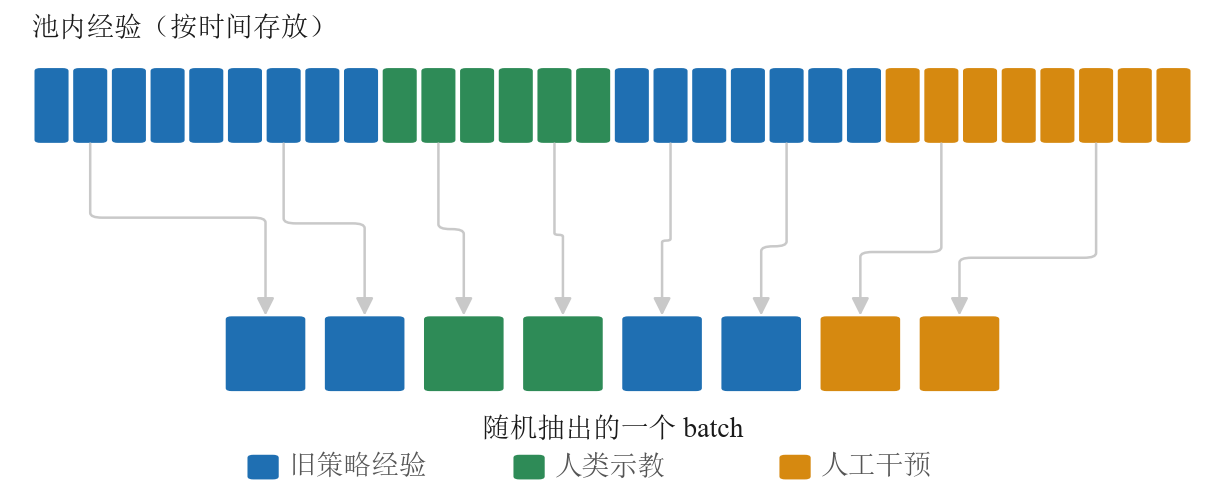
\includegraphics[width=1\linewidth,height=\textheight,keepaspectratio]{../../assets/figures/lecture16/ref/fig162-replay-buffer.png}

}

\caption{经验池的存与取：上排为按时间存放的池内转移（来源成片、相邻相关），下排为随机抽出的一个
batch（时刻与来源全打散）}

\end{figure}%

上图把''存''和''取''画在了一起：上排是池子的真实存放顺序------按时间一条条排过去，同一段颜色（同一来源、同一回合）连成片，相邻两条转移几乎长一样；下排是训练时真正喂给网络的一个
batch------从池子里随机翻牌抽出来，蓝、绿、黄混在一起，时间顺序也乱了。网络每一步看到的都是这样一把''混装''的经验，梯度自然稳。

对照第14讲的 PPO 就能看清差别：PPO
的''数据仓库''每轮清空重建，本质是\textbf{缓冲区}；replay buffer
只进不清（满了才挤掉最旧的），是真正的\textbf{资产}。HIL-SERL
还会维护两个池子------在线经验一个、人类示教一个------那是第 8
节的事，机制完全相同。

\subsection{2.3 Q
函数：给「状态-动作」记账}\label{q-ux51fdux6570ux7ed9ux72b6ux6001-ux52a8ux4f5cux8bb0ux8d26}

off-policy
为什么能不挑数据来源？根子在它学的东西不一样。策略梯度直接学''该做什么''，而价值方法先学''\textbf{做了会怎样}''。

第14讲 2.4 节我们已经认识了价值函数 \(V(s)\)------``从状态 \(s\)
出发平均还能拿多少回报''。但 \(V\)
有个先天短板：它把''之后会怎么做''整个托付给了某个策略，所以它天生绑定那个策略------换个策略，同一个状态的
\(V\) 就变了，旧策略采的数据也就没法直接给新策略估 \(V\)。off-policy
需要一个更''钉得死''的对象：把\textbf{第一步的动作也固定下来}------

\[Q(s, a) = \text{从状态 } s \text{ 做动作 } a \text{ 出发，之后平均还能拿多少回报}\]

\(Q\) 比 \(V\) 多钉住一个动作，好处立竿见影：一条数据 \((s, a, \ldots)\)
里的 \(s\) 和 \(a\) 都是\textbf{既成事实}，不管这个 \(a\)
是谁选的------旧策略、人手、随机探索------``在 \(s\) 做了
\(a\)''这件事对任何人都是同一件事。评价既成事实，不需要征得当事策略的同意。

写成式子就是：

\[
Q^\pi(s,a)=\mathbb{E}_{\pi}\big[\,r_{t+1}+\gamma r_{t+2}+\gamma^2 r_{t+3}+\cdots \,\mid\, s_t=s,\ a_t=a\,\big]
\]

逐段读一遍：等号左边是''这个状态-动作对值多少''；右边的期望是''未来能拿到的折扣回报''；竖线后面挂着两个条件------\textbf{从状态
\(s\) 出发}，\textbf{并且第一步做动作 \(a\)}；而期望下标的 \(\pi\)
在提醒我们，第一步之后的每一步仍然按策略 \(\pi\) 走。和第14讲 5.2 节的
\(V^\pi(s)\) 相比，唯一多出来的就是''第一步做了 \(a\)``这个条件。

这个 \(Q\)
函数不是靠完整轨迹的总回报学的，而是靠\textbf{自举（bootstrap）}------用下一步的估值来更新这一步（第14讲
5.3 节我们用它区分过 REINFORCE 和 Actor-Critic）。对每一条转移记录
\((s, a, r, s')\)，\(Q\) 应该满足：

\[y = r + \gamma \,(1 - d)\, Q(s', a'), \qquad a' \sim \pi(\cdot \mid s')\]

\begin{center}
\begin{tabular}{@{}>{\raggedright\arraybackslash}p{\dimexpr 0.1355\linewidth - 2\tabcolsep\relax} >{\raggedright\arraybackslash}p{\dimexpr 0.5878\linewidth - 2\tabcolsep\relax} >{\raggedright\arraybackslash}p{\dimexpr 0.2767\linewidth - 2\tabcolsep\relax}@{}}
\toprule\noalign{}
符号 & 含义 & 典型取值 \\
\midrule\noalign{}
\((s, a, r, s')\) & 一条转移：状态、动作、即时奖励、下一状态 & 来自 replay buffer \\
\(y\) & \(Q(s,a)\) 的更新目标 & --- \\
\(\gamma\) & 折扣因子 & 0.99 \\
\(d\) & 回合是否在 \(s'\) 终止（终止则不再有后续回报） & 0 或 1 \\
\(a'\) & 由\textbf{当前}策略在 \(s'\) 处选出的下一动作 & --- \\
\bottomrule\noalign{}
\end{tabular}
\end{center}

注意这个等式的一个关键性质：它对\textbf{任何来源}的转移
\((s, a, r, s')\)
都成立。这条转移是三天前的旧策略采的、是人示教的、还是干预时人打的方向，都不影响''\(s\)
做 \(a\) 得了 \(r\) 到了 \(s'\)``这个事实------下一步的动作 \(a'\)
用\textbf{当前策略}重新选就行。\textbf{这就是 off-policy
能吃百家饭的数学根源}：贝尔曼等式描述的是环境的因果，而不是某个策略的偏好。

价值方法还有一个对真机特别重要的本事：\textbf{把稀疏的成功传播开}。真机任务的奖励往往只有''最后成没成功''一个
0/1 信号（第 8
节会看到它甚至是学出来的）。策略梯度面对这种奖励几乎摸不到方向；而 \(Q\)
函数靠自举，能像多米诺骨牌一样把终点的信号一格一格传回起点。

用一个迷你例子把''传播''演出来。假设推方块任务的一个成功回合只有三步，产生三条转移进池子（\(\gamma = 0.9\)，\(Q\)
初始全为 0）：

\begin{center}
\begin{tabular}{@{}>{\raggedright\arraybackslash}p{\dimexpr 0.0938\linewidth - 2\tabcolsep\relax} >{\raggedright\arraybackslash}p{\dimexpr 0.4375\linewidth - 2\tabcolsep\relax} >{\raggedright\arraybackslash}p{\dimexpr 0.0938\linewidth - 2\tabcolsep\relax}@{}}
\toprule\noalign{}
转移 & 内容 & 奖励 \\
\midrule\noalign{}
甲 & \((s_0, a_0, 0, s_1)\)：伸向方块 & 0 \\
乙 & \((s_1, a_1, 0, s_2)\)：抵住方块推 & 0 \\
丙 & \((s_2, a_2, 1, \text{终止})\)：方块进目标区 & 1 \\
\bottomrule\noalign{}
\end{tabular}
\end{center}

训练时反复从池子里随机抽转移，看 \(Q\) 值怎么演化：

\begin{itemize}
\tightlist
\item
  第一次抽到\textbf{丙}：终止转移，目标 \(y = 1\)，于是 \(Q(s_2, a_2)\)
  朝 1 更新------成功本身先被记住。
\item
  之后抽到\textbf{乙}：目标
  \(y = 0 + 0.9 \times Q(s_2, a_2) \approx 0.9\)------虽然乙自己的奖励是
  0，但''它通向一个值 1 的地方''这件事通过自举传了过来，\(Q(s_1, a_1)\)
  朝 0.9 涨。
\item
  再抽到\textbf{甲}：同理 \(Q(s_0, a_0)\) 朝
  \(0.9 \times 0.9 \approx 0.81\) 涨。
\end{itemize}

\begin{figure}[H]

{\centering 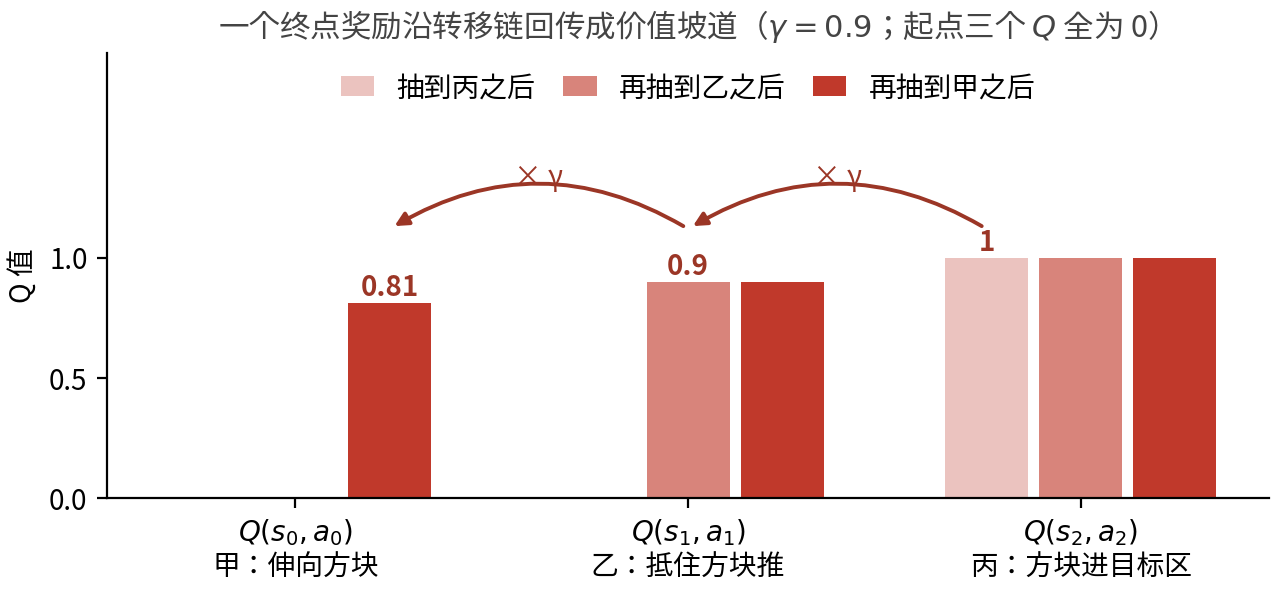
\includegraphics[width=0.88\linewidth,height=\textheight,keepaspectratio]{../../assets/figures/lecture16/ref/fig162-q-propagation.png}

}

\caption{稀疏的终点奖励沿转移链回传：抽到丙记住成功，再抽到乙、甲时价值按
\(\gamma\) 折扣逐格向起点传播，长成一条价值坡道}

\end{figure}%

上图把这三轮抽样画成了柱状图：最初三根柱子全是零；抽到丙后最右边先立起来（值
1）；随后每次自举都把价值乘上 \(\gamma\)
往左传一格------0.9、0.81。几轮下来，一个孤零零的终点奖励就被摊开成了一条\textbf{从起点到终点逐渐升高的价值坡道}，后面的
actor
只要顺着坡爬就行。注意整个过程对抽样顺序、对这三条转移是谁采的都没有要求------早抽到乙也没关系（那时目标还是
0，等丙学进去后乙迟早会被再次抽到）；池子里随机翻牌，信号自然回流。

\begin{quote}
备注：目标 \(y\)
里还有一个不起眼但关键的工程件------\textbf{目标网络}。如果 \(y\) 里的
\(Q(s', a')\)
用的是正在被训练的同一个网络，那么每次参数更新，所有目标值都跟着晃，网络等于在追自己的尾巴。实践中会维护一份\textbf{延迟拷贝}
\(\bar{Q}\) 专门算目标：每步只让它朝主网络挪一小步（软更新，比例
\(\tau \approx 0.005\)）。目标稳住了，回归才收敛。上面公式里的
\(Q(s', a')\)，实现中都读作 \(\bar{Q}(s', a')\)。
\end{quote}

\subsection{2.4 动手：CartPole
上从查表到用网络}\label{ux52a8ux624bcartpole-ux4e0aux4eceux67e5ux8868ux5230ux7528ux7f51ux7edc}

前面 Q
函数、经验池、目标网络都还是纸面概念。在上真机、上机械臂之前，先用一个最小的任务把它们\textbf{跑成代码}------经典的
CartPole：一根杆立在小车上，左右推车让杆不倒，动作只有''左推 /
右推''两个离散选项。它简单到能在几分钟内训完，却正好能把''从查表到用网络''这一步演清楚。

\subsubsection{任务}\label{ux4efbux52a1}

CartPole
的观测是四个连续量（小车位置、小车速度、杆的角度、杆的角速度），动作只有''左推
/ 右推''两个；每活一步得 1 分，杆倒或小车出界即回合结束，单回合最高 500
分。两个版本用同一个任务、同一套统计口径（回合回报），\textbf{版本之间的差异就是这一节的知识点}。

\subsubsection{第一版：表格
Q-learning}\label{ux7b2cux4e00ux7248ux8868ux683c-q-learning}

最朴素的做法是给每个''状态-动作''配一格账，存成一张表。可连续值没法当表格的下标------于是第一步永远是\textbf{分桶}：每一维切成
8 段，四维组合起来就是表的''状态''维度（\(8^4 \times 2\)
格）。然后就是上一节那套 Q 更新，逐格填表，\(\varepsilon\)-greedy
采样（大概率按当前最优、小概率随机试）：

\begin{Shaded}
\begin{Highlighting}[]
\NormalTok{        cell }\OperatorTok{=} \BuiltInTok{tuple}\NormalTok{(state.tolist()) }\OperatorTok{+}\NormalTok{ (}\BuiltInTok{int}\NormalTok{(action),)}
\NormalTok{        best\_next }\OperatorTok{=} \VariableTok{self}\NormalTok{.model.table[}\BuiltInTok{tuple}\NormalTok{(next\_state.tolist())].}\BuiltInTok{max}\NormalTok{()}
\NormalTok{        target }\OperatorTok{=}\NormalTok{ reward }\OperatorTok{+} \VariableTok{self}\NormalTok{.gamma }\OperatorTok{*}\NormalTok{ best\_next }\OperatorTok{*}\NormalTok{ (}\FloatTok{1.0} \OperatorTok{{-}}\NormalTok{ done)}
\NormalTok{        td\_error }\OperatorTok{=}\NormalTok{ target }\OperatorTok{{-}} \VariableTok{self}\NormalTok{.model.table[cell]}

        \CommentTok{\# 这一行就是表格 Q{-}learning 的全部：把这一格往目标挪 ALPHA 那么多。}
        \VariableTok{self}\NormalTok{.model.table[cell] }\OperatorTok{+=} \VariableTok{self}\NormalTok{.alpha }\OperatorTok{*}\NormalTok{ td\_error}
\end{Highlighting}
\end{Shaded}

这一版\textbf{没有神经网络}------``没有网络''本身就是要暴露的教学点。Q
表放在一个 \texttt{nn.Module}
里，但里面一个可训练参数都没有，整张表只是个
buffer；既然没有梯度，优化器自然也没有：

\begin{Shaded}
\begin{Highlighting}[]
    \KeywordTok{def} \FunctionTok{\_\_init\_\_}\NormalTok{(}\VariableTok{self}\NormalTok{, n\_actions):}
        \BuiltInTok{super}\NormalTok{().}\FunctionTok{\_\_init\_\_}\NormalTok{()}
        \CommentTok{\# register\_buffer：随模型保存/加载，但不是可训练参数。}
        \VariableTok{self}\NormalTok{.register\_buffer(}\StringTok{"table"}\NormalTok{, torch.zeros((NUM\_BINS,) }\OperatorTok{*} \DecValTok{4} \OperatorTok{+}\NormalTok{ (n\_actions,)))}
        \VariableTok{self}\NormalTok{.n\_actions }\OperatorTok{=}\NormalTok{ n\_actions}
\end{Highlighting}
\end{Shaded}

既然没有梯度，优化器也就无从谈起------\texttt{configure\_optimizers}
直接返回空：

\begin{Shaded}
\begin{Highlighting}[]
    \KeywordTok{def}\NormalTok{ configure\_optimizers(}\VariableTok{self}\NormalTok{):}
        \CommentTok{\# 查表更新不是梯度下降，这里确实没有优化器可配。}
        \ControlFlowTok{return} \VariableTok{None}
\end{Highlighting}
\end{Shaded}

表格法的致命短板是：状态得手工分桶，而表的大小是\textbf{每维桶数的连乘}。四维还能勉强切，换成图像或机械臂几十维的状态，桶数直接组合爆炸、根本存不下------这就是''维度诅咒''。

\subsubsection{第二版：DQN}\label{ux7b2cux4e8cux7248dqn}

解法是把那张表换成一个\textbf{神经网络}：输入原始连续状态，输出每个动作的
Q
值。网络能在相近状态之间\textbf{泛化}，不用穷举分桶，天然绕开维度爆炸------这种''用一个可学习的函数去近似整张
Q 表''的做法叫\textbf{函数近似}。

但网络不能像表格那样即采即改：训练样本前后高度相关、更新目标自己还在动，直接套表格那套会训崩。于是把上两节攒下的两件工程配件正式装上------\textbf{经验回放}（2.2
节，随机抽 batch 打断相关性）和\textbf{目标网络}（2.3
节备注，稳住回归目标）。三处改动一目了然：

\begin{Shaded}
\begin{Highlighting}[]
\NormalTok{        q\_values }\OperatorTok{=} \VariableTok{self}\NormalTok{.online(states).gather(}\DecValTok{1}\NormalTok{, actions.unsqueeze(}\DecValTok{1}\NormalTok{)).squeeze(}\DecValTok{1}\NormalTok{)}
        \ControlFlowTok{with}\NormalTok{ torch.no\_grad():}
            \CommentTok{\# 采集时 dones 写的是 terminated（不含 truncated），}
            \CommentTok{\# 所以真正失败才不 bootstrap，这里直接乘 (1 {-} dones)。}
\NormalTok{            next\_q }\OperatorTok{=} \VariableTok{self}\NormalTok{.target(next\_states).}\BuiltInTok{max}\NormalTok{(dim}\OperatorTok{=}\DecValTok{1}\NormalTok{).values}
\NormalTok{            td\_target }\OperatorTok{=}\NormalTok{ rewards }\OperatorTok{+} \VariableTok{self}\NormalTok{.gamma }\OperatorTok{*}\NormalTok{ next\_q }\OperatorTok{*}\NormalTok{ (}\FloatTok{1.0} \OperatorTok{{-}}\NormalTok{ dones)}
\NormalTok{        loss }\OperatorTok{=}\NormalTok{ nn.functional.mse\_loss(q\_values, td\_target)}
\end{Highlighting}
\end{Shaded}

对着上一版读：Q 值的来源从 \texttt{table{[}s{]}} 变成了
\texttt{online(s)}，查表变成了前向计算；算目标用的是
\texttt{self.target} 而不是
\texttt{self.online}，一份延迟拷贝专门负责给出回归目标，网络不再追自己的尾巴；最后，更新不再是改表里的一格，而是对\textbf{一整个
minibatch} 做回归------而这个 batch
来自经验池的随机抽样，正好把同一条轨迹上前后相邻的样本打散。

两版的骨架完全一样（在线采样的 \texttt{Dataset} →
\texttt{LightningDataModule} → \texttt{nn.Module} →
\texttt{LightningModule}，入口都是 \texttt{trainer.fit}），换掉的只有''Q
从哪来''。

\subsubsection{结果}\label{ux7ed3ux679c}

两版各跑一次，横轴统一用环境步数（两级的回合长度差很多，按回合数对齐会误导）：

\begin{figure}[H]

{\centering 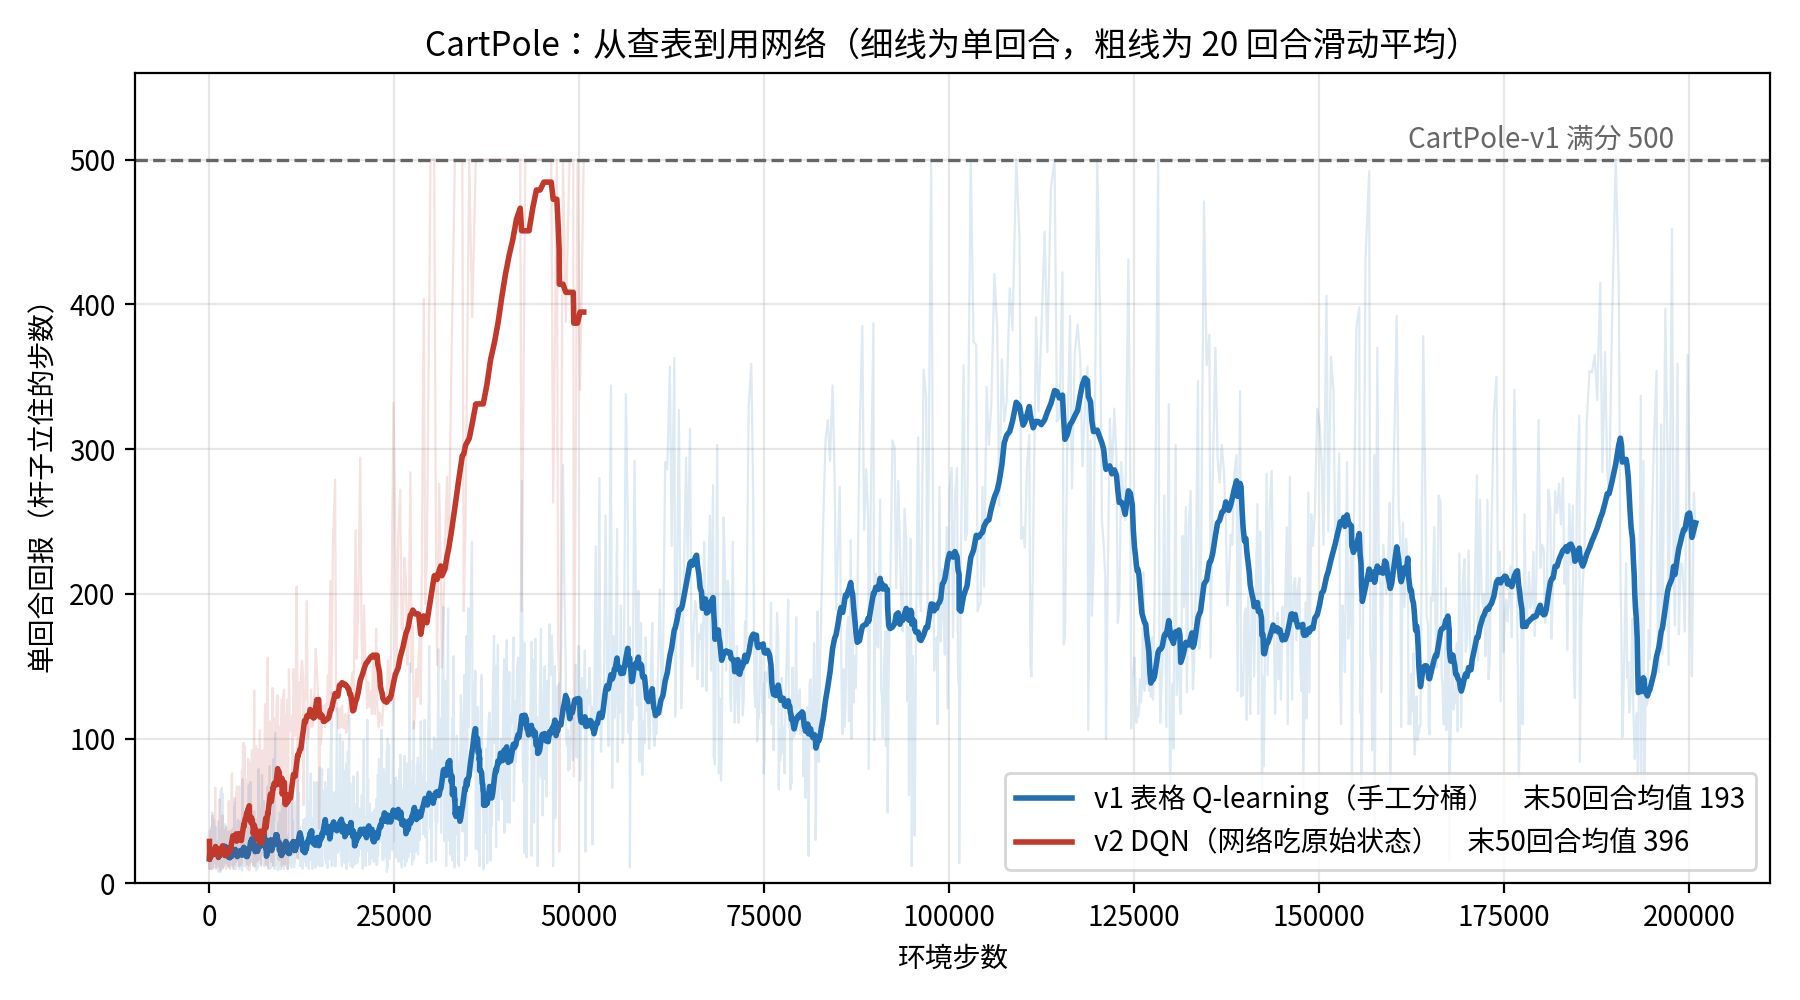
\includegraphics[width=0.96\linewidth,height=\textheight,keepaspectratio]{../../assets/figures/lecture16/ref/fig162-cartpole-returns.png}

}

\caption{CartPole 两级值学习的回合回报对照：v1 表格 Q-learning 跑满 20
万步也没稳住，滑动均值一路在 100～350 分之间起落、收在 193 分；v2 DQN 约
3 万步就打出第一个 500 分满分回合，5 万步收工时末 50 回合里已有 31
个满分}

\end{figure}%

\begin{center}
\begin{tabular}{@{}>{\raggedright\arraybackslash}p{\dimexpr 0.0795\linewidth - 2\tabcolsep\relax} >{\raggedright\arraybackslash}p{\dimexpr 0.3572\linewidth - 2\tabcolsep\relax} >{\raggedright\arraybackslash}p{\dimexpr 0.1349\linewidth - 2\tabcolsep\relax} >{\raggedright\arraybackslash}p{\dimexpr 0.2521\linewidth - 2\tabcolsep\relax} >{\raggedright\arraybackslash}p{\dimexpr 0.1761\linewidth - 2\tabcolsep\relax}@{}}
\toprule\noalign{}
版本 & 方法 & 环境步数 & 末 50 回合平均回报 & 其中满分回合 \\
\midrule\noalign{}
v1 & 表格 Q-learning（手工分桶） & 20.1 万 & 193 & 0 / 50 \\
\textbf{v2} & \textbf{DQN（网络吃原始状态）} & \textbf{5.0 万} & \textbf{396} & \textbf{31 / 50} \\
\bottomrule\noalign{}
\end{tabular}
\end{center}

差距很干脆：\textbf{DQN
只用了表格法四分之一的交互，成绩却是它的两倍}。末段的质量差得更远------DQN
最后 50 个回合里有 31 个直接打满 500
分，表格法一个都没有，最好的一次也只到 452。

原因就在分桶。每维只切 8
段，落进同一个桶的状态被当成同一个状态------杆子偏 3° 和偏 8° 共用一格 Q
值，策略再怎么训也精细不到哪去；而且相邻桶之间没有任何信息共享，每一格都得自己撞够次数才学得会。DQN
的网络恰恰相反：相近的状态天然给出相近的 Q
值，一次更新就能惠及一片邻域，所以又快又稳。

\textbf{这就是''函数近似''四个字的实际含义}：不是换了个更聪明的更新公式，而是换了一种''记住经验''的方式------记得越会举一反三，同样的交互量就换得回越高的回报。

不过省样本从来不是白省的。函数近似、自举、off-policy
这三样一旦凑齐，训练就失去了''只会越来越好''的保证------下一节就来算这笔账。

到这里，Q 函数、经验池、目标网络都从概念变成了能跑的代码。但 DQN
还卡着一道坎：它靠''对每个动作的 Q 取
\textbf{argmax}''来选动作，这只在动作是\textbf{有限几个离散选项}时才做得到。机械臂的动作是六个关节的连续力矩------argmax
无从枚举。要把 off-policy 带上机械臂，就得换一类''不靠
argmax、直接吐连续动作''的算法。而在动手爬这条连续控制的阶梯之前，还得先认清
off-policy 省下样本要付的那份代价。

\subsection{2.5 天下没有免费的午餐：off-policy
的稳定性代价}\label{ux5929ux4e0bux6ca1ux6709ux514dux8d39ux7684ux5348ux9910off-policy-ux7684ux7a33ux5b9aux6027ux4ee3ux4ef7}

既然 off-policy
这么省样本，第14讲为什么不直接教它？因为它天生更难训稳。强化学习里有个著名的''\textbf{死亡三角}''：\textbf{自举}、\textbf{函数近似}（神经网络）、\textbf{离策略数据}------三者单独都没事，凑齐了就容易让训练发散：

\begin{center}
\begin{tabular}{@{}>{\raggedright\arraybackslash}p{\dimexpr 0.2705\linewidth - 2\tabcolsep\relax} >{\raggedright\arraybackslash}p{\dimexpr 0.3670\linewidth - 2\tabcolsep\relax} >{\raggedright\arraybackslash}p{\dimexpr 0.3625\linewidth - 2\tabcolsep\relax}@{}}
\toprule\noalign{}
组合 & 熟悉的例子 & 稳吗 \\
\midrule\noalign{}
只有函数近似 & 监督学习 & 稳：标签固定，回归目标不动 \\
自举 + 离策略，无函数近似 & 表格型 Q-learning（每个状态一格） & 稳：有收敛保证 \\
函数近似 + 自举，on-policy & 第14讲 A2C/PPO 的 critic & 基本稳：数据新鲜，错账很快被重访修正 \\
三者齐 & 深度 off-policy（本讲） & 要靠工程兜底 \\
\bottomrule\noalign{}
\end{tabular}
\end{center}

三者凑齐为什么危险？直觉是：\(Q\)
用自己的估值更新自己（自举），估值本身有误差（网络近似），而离策略数据又让''账本出错的地方''和''账本被查账的地方''错开------网络在池子里那批旧数据上改账本，改动却会牵连到当前策略常去的状态（函数近似让相邻状态的估值联动），那些地方的错误迟迟等不到新数据来纠正，误差就可能越滚越大。

on-policy
方法（PPO）用''只吃新鲜数据''砍掉了第三条边，所以稳，代价是费样本；off-policy
方法三条边全占，所以省样本，代价是要靠一堆工程手段兜底。这些兜底手段------双
Q
取小（治高估）、目标网络软更新（治追尾巴）、随机抽样（治样本相关）、合适的更新采样比（UTD，update-to-data
ratio，即每采一步数据做几次梯度更新，治更新过猛）------下面几章会在
SO-101
阶梯上逐级登场：哪一级栽了跟头、要补哪一件配件，都对着死亡三角的某一条边。它们不是装饰，本讲后面的方法（DDPG、TD3、SAC、HIL-SERL）都带着这样一串''稳定性配件''。

\subsection{2.6 与上一讲的分水岭：critic
请走了，又请回来}\label{ux4e0eux4e0aux4e00ux8bb2ux7684ux5206ux6c34ux5cadcritic-ux8bf7ux8d70ux4e86ux53c8ux8bf7ux56deux6765}

第15讲我们刚把 critic 请走（GRPO
用组内平均分当基线），这一讲怎么又请回来了？对照一下两边的处境就清楚了：

\begin{center}
\begin{tabular}{@{}>{\raggedright\arraybackslash}p{\dimexpr 0.2295\linewidth - 2\tabcolsep\relax} >{\raggedright\arraybackslash}p{\dimexpr 0.3711\linewidth - 2\tabcolsep\relax} >{\raggedright\arraybackslash}p{\dimexpr 0.3994\linewidth - 2\tabcolsep\relax}@{}}
\toprule\noalign{}
 & 第15讲（GRPO 后训练） & 第16讲（真机 RL） \\
\midrule\noalign{}
动作 & 离散 token，一次生成一段 & 连续控制量，10 Hz 逐步闭环 \\
奖励 & 可验证：规则一判就有 & 稀疏 0/1，还得靠视觉判 \\
一组采样的成本 & 便宜（GPU 上采一组回答） & 昂贵（真机跑一组 rollout） \\
数据能否复用 & 不复用也无妨 & 必须复用 \\
基线/信号 & 组内比较就够 & 要靠 \(Q\) 自举把稀疏信号传开 \\
\bottomrule\noalign{}
\end{tabular}
\end{center}

GRPO 免 critic 的前提是''同题采一组很便宜''；真机上一组 rollout
本身就是最贵的东西，而且连续动作加稀疏奖励，光靠组内比较传播不了信号。所以
critic 回来了，而且这次它是主角：\textbf{off-policy
的一切复用能力，都建立在 \(Q\) 函数这本''不挑数据来源的账''上}。

\subsection{2.7 本节小结}\label{ux672cux8282ux5c0fux7ed3-1}

本节建立了这一讲的方法底座。off-policy
的定义是行为策略与目标策略解耦，由此旧数据、人类示教、人工干预都成为合法训练数据，统一存进
replay buffer 这座''资产仓库''随机取用；数学根源是 \(Q\)
函数评价的是''在 \(s\) 做了
\(a\)``这个既成事实，贝尔曼等式对任何来源的转移都成立。\(Q\)
靠自举把稀疏的成功信号沿价值坡道一格格传回起点，目标网络稳住回归目标。我们在
CartPole 上把这套概念跑成了代码------从手工分桶的表格
Q，到用神经网络吃原始状态的 DQN，''函数近似 + 经验回放 +
目标网络''就此凑齐。但 DQN 靠 argmax
选动作，迈不进连续控制；而三者一凑齐，死亡三角带来的稳定性风险也一并到场。接下来我们就在
SO-101 上从零爬一条 off-policy
阶梯，一级一级把连续动作和稳定性这两道坎补上------这也是为什么入门先学
on-policy，上真机才换 off-policy。

\section{3
DDPG：把确定性策略带进连续动作}\label{ddpgux628aux786eux5b9aux6027ux7b56ux7565ux5e26ux8fdbux8fdeux7eedux52a8ux4f5c}

前面 CartPole 上的 DQN 有一个天花板：它靠''对每个动作的 Q 值取
argmax''来选动作，这只在动作是\textbf{有限几个离散选项}时才做得到。可
SO-101 机械臂的动作是六个关节的连续力矩，把连续区间切成格子再
argmax，格子数随维度指数爆炸------和上一节表格 Q
撞的是同一堵墙。要在连续动作空间里做
off-policy，得换一个思路：不再''评分选最高''，而是\textbf{直接让一个网络吐出动作}。这就是
DDPG。

从这一章起，我们把战场搬到 SO-101
的仿真环境，用同一个任务、同一套训练预算，只换算法，一级级往上爬------就像第14讲在
G1 行走上从 REINFORCE 爬到 PPO
一样，\textbf{每一级和上一级的差异，就是这一节的知识点}。

\subsection{3.1
任务与环境：一个''够到方块''的最小操作}\label{ux4efbux52a1ux4e0eux73afux5883ux4e00ux4e2aux591fux5230ux65b9ux5757ux7684ux6700ux5c0fux64cdux4f5c}

四级算法都在同一个任务上比：\textbf{SO101ReachCube}------机械臂把末端够到桌上的方块。这是操作任务里最简单的一档（纯靠近，不用抓取），却已经足够暴露每个算法的脾气。

\begin{figure}[H]

{\centering 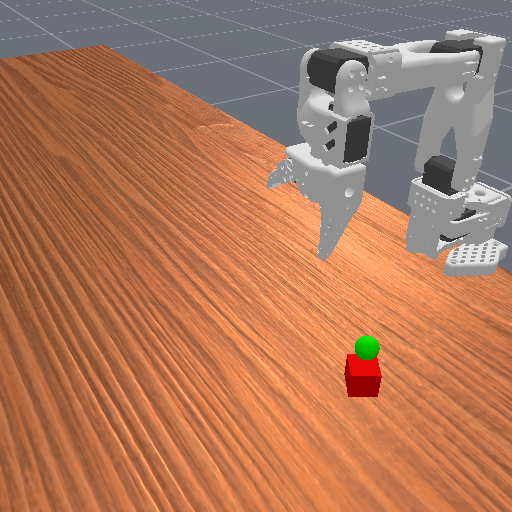
\includegraphics[width=0.6\linewidth,height=\textheight,keepaspectratio]{../../assets/figures/lecture16/ref/fig-so101-reachcube-scene.png}

}

\caption{SO-101 机械臂与 ReachCube 任务：低成本的 SO-101
臂要把末端够到桌面上的方块，红块顶端的绿色小球是目标标记。这套仿真场景与
VLA 课评测、复现数据用的是同一个环境}

\end{figure}%

环境复用的正是 VLA 课用过的那套 SO-101
仿真（\texttt{so101\_sim}）。这里先记住一个贯穿全讲的事实：\textbf{强化学习训练用的环境，和
VLA
课评测、复现数据用的，是同一个环境}------只是这里开一千个并行实例快速采样，VLA
那边开一个实例做评测。等爬到第 6 级
squint，我们会看到这条线怎么闭合成一整个数据闭环。

策略看到的观测是关节状态（位置、速度、物体位姿等，共 55
维），动作是六维连续量。奖励是\textbf{稠密}的：末端离方块越近，每一步给的奖励越高。稠密奖励很重要------它给了算法一个连续的''往哪走更好''的信号，不像''够到才
+1''那样一片荒漠。

\subsection{3.2 DDPG 的两个网络：Actor 出动作，Critic
打分}\label{ddpg-ux7684ux4e24ux4e2aux7f51ux7edcactor-ux51faux52a8ux4f5ccritic-ux6253ux5206}

DDPG（Deep Deterministic Policy Gradient）的骨架是两个网络：

\begin{itemize}
\tightlist
\item
  \textbf{Actor}（确定性策略）：输入状态，直接输出一个确定的动作（六维力矩），末端用
  \texttt{tanh} 把动作压进合法区间。它不像上一讲 PPO
  那样输出一个概率分布再采样，而是''看到这个状态，我就做这个动作''。
\item
  \textbf{Critic}（Q 网络）：输入''状态 + 动作''，输出一个标量 Q
  值，即''在这个状态做这个动作，预计能拿多少回报''。这就是上一节 Q
  函数的连续版------DQN 的 Q 网络对每个离散动作出一个分，DDPG 的 Critic
  直接把动作当输入吃进去出一个分。
\end{itemize}

两者怎么配合训练？

\begin{itemize}
\tightlist
\item
  \textbf{Critic 学法}和 DQN 一脉相承：用贝尔曼目标
  \(r + \gamma\, Q_{\text{target}}(s', \pi(s'))\) 做回归，只是下一动作由
  Actor（而非 argmax）给出，同样配一套缓慢跟随的目标网络。
\item
  \textbf{Actor 学法}是 DDPG
  的点睛之笔，叫\textbf{确定性策略梯度}：Actor 要让 Critic
  给自己打的分越高越好，于是损失就是 \(-Q(s, \pi(s))\)。梯度顺着 Critic
  一路回传到 Actor------\textbf{Critic 告诉
  Actor''往动作空间的哪个方向挪，我给的分会更高''，Actor 就照着挪}。
\end{itemize}

探索呢？确定性策略自己不带随机性，DDPG
靠在输出动作上\textbf{外加一点高斯噪声}来试探周围。记住这个''外加噪声''------它后面会成为整条阶梯的命门。

代码上这就是标准的四件套：\texttt{DeterministicActor} 和
\texttt{QCritic} 两个 \texttt{nn.Module}，\texttt{DDPG} 这个
\texttt{LightningModule} 在一个 minibatch 里先更新 Critic、再更新
Actor、最后软更新目标网络（\texttt{train\_v3\_ddpg.py}）。

\begin{figure}[H]

{\centering 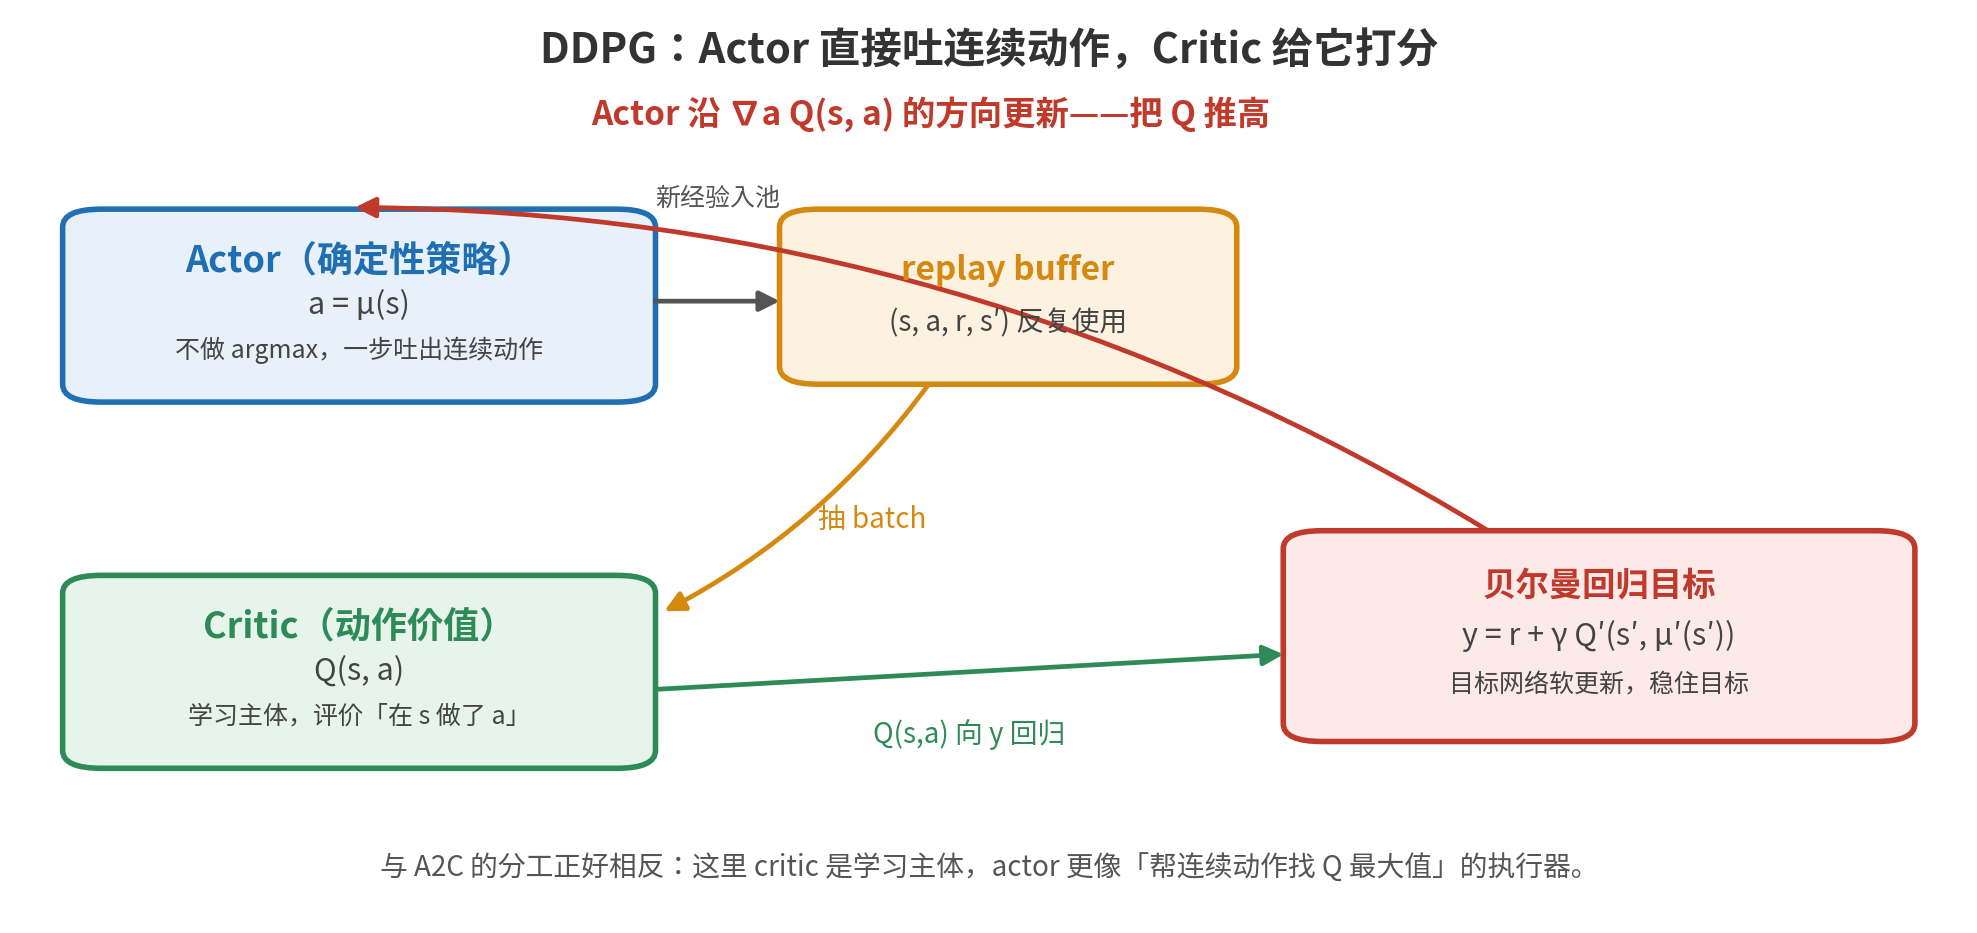
\includegraphics[width=0.8\linewidth,height=\textheight,keepaspectratio]{../../assets/figures/lecture16/ref/fig162-actor-critic-ddpg.png}

}

\caption{DDPG 的 Actor-Critic 分工：actor 直接吐出连续动作
\(a=\mu(s)\)，critic 学 \(Q(s,a)\) 并沿 \(\nabla_a Q\) 指导 actor；与
A2C 相反，这里 critic 是学习主体}

\end{figure}%

这张图就是 DDPG 两个网络的分工：Actor 看状态吐出动作，Critic
给''这个状态下这个动作''打分，再把''往动作空间哪个方向挪能让分更高''的梯度回传给
Actor------上面确定性策略梯度那一步，在图上就是这条从 Critic 指回 Actor
的箭头。

\subsection{3.3
一个真实的坑：不归一化，网络直接学不动}\label{ux4e00ux4e2aux771fux5b9eux7684ux5751ux4e0dux5f52ux4e00ux5316ux7f51ux7edcux76f4ux63a5ux5b66ux4e0dux52a8}

第一次把 DDPG 跑起来，结果是\textbf{成功率全程
0，而且平均奖励一动不动}------像下面这条红线，从头到尾在原地打转。

按常理，DDPG
是成熟算法、奖励又是稠密的，不该毫无起色。我们顺着查下去，查出一个非常具体、也非常典型的病根，值得当作一个案例讲透。

第一步先排除''是不是训练不够''：把并行环境加到一千、每步更新加到 256
次、探索噪声调大，甚至照 DDPG
原论文给末层用小初始化------\textbf{统统还是 0}。这说明不是预算问题。

第二步盯住 Actor 的\textbf{权重范数}看：它 600
次迭代下来，数值一位小数都不变。这是一个强信号------\textbf{Actor
根本没在更新}，梯度约等于零。

第三步找零梯度的来源。回头看观测：SO-101 的状态里有的分量数值到了
\textbf{200}
这个量级（比如某些位姿读数），而且没有做任何归一化。这么大的数直接喂进
Actor 的 MLP，逐层放大，到末端 \texttt{tanh}
时早已\textbf{深度饱和}------而 \texttt{tanh}
在饱和区的梯度几乎为零。梯度在这里被掐断，Actor
于是冻在初始值上，成功率自然永远是 0。

修法是强化学习里的标准动作，你在第14讲的 G1
代码里其实已经见过：\textbf{观测归一化}。在线统计每一维观测的均值和方差，把状态归一化到零均值、单位方差再喂网络，大数值就不会把
\texttt{tanh} 顶进饱和区。加上这一步，Actor
的权重立刻开始更新，平均奖励也从''死平''变成''在涨''：

\begin{figure}[H]

{\centering 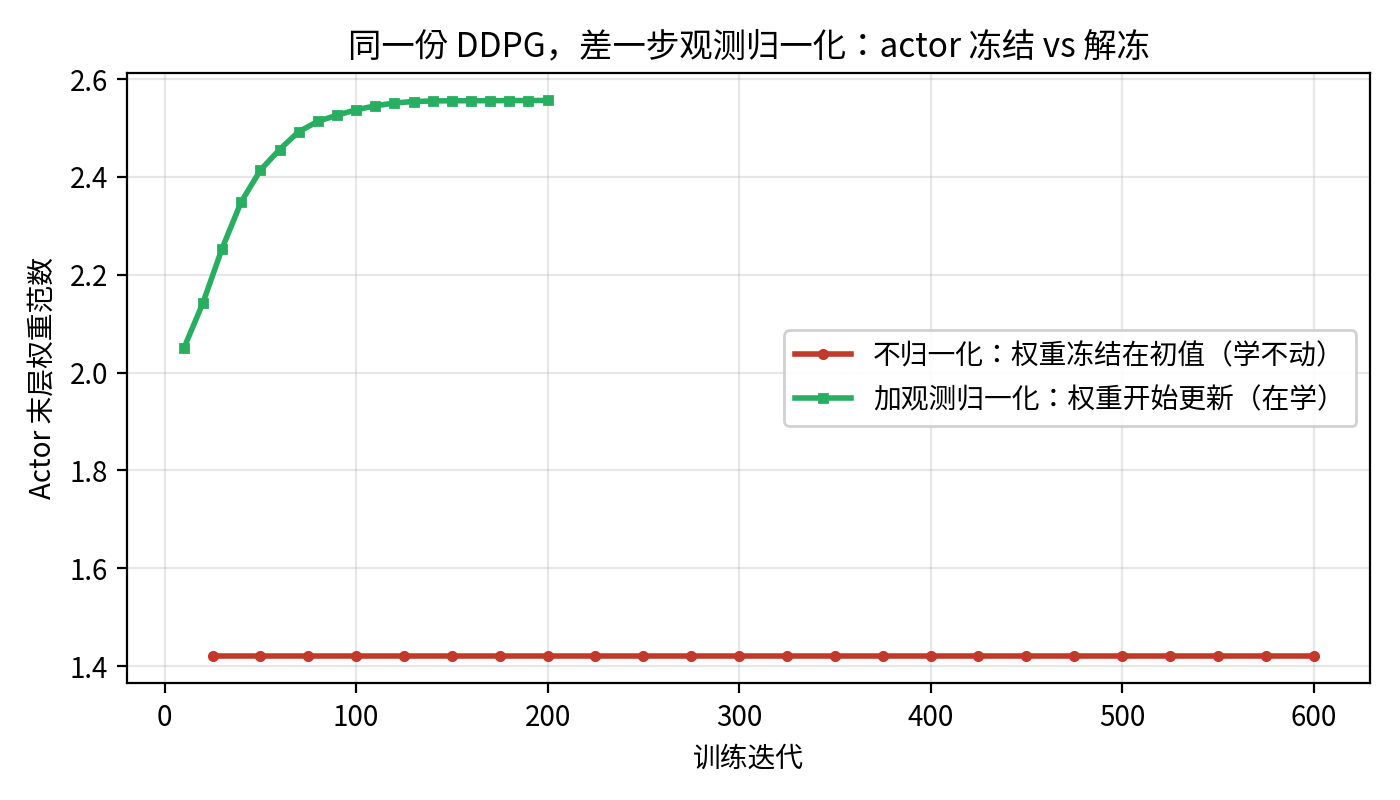
\includegraphics[width=0.85\linewidth,height=\textheight,keepaspectratio]{../../assets/figures/lecture16/ref/fig-obsnorm-freeze.png}

}

\caption{同一份 DDPG，只差一步观测归一化：不归一化时 Actor 末层权重范数
600
次迭代冻在初值（红线，学不动），加上在线观测归一化后权重开始更新（绿线，在学）}

\end{figure}%

\begin{quote}
备注：为什么第 6 级 squint（下文）不需要单独加这一步？因为它的网络里用了
LayerNorm，等于把归一化揉进了结构里。归一化不是可有可无的调参，是让梯度能正常流动的前提------这一点对\textbf{任何}拿原始观测喂
MLP
的连续控制都成立，回到第8讲讲部署时反复强调的''数值口径要对齐''是同一个道理。
\end{quote}

这个插曲的价值不在 bug
本身，而在它演示了\textbf{怎么诊断一个''学不动''的强化学习}：先排除预算、再定位是哪个网络没动、再顺着零梯度找到数值根因。真机上遇到''怎么训都不涨''，走的就是这条路。

\subsection{3.4 DDPG
的成绩与毛病}\label{ddpg-ux7684ux6210ux7ee9ux4e0eux6bdbux75c5}

归一化修好后，DDPG 在 ReachCube
上终于开始学------但学得\textbf{很不稳}。看章首那条红线：平均奖励在剧烈震荡，一会儿爬上去、一会儿又栽下来，始终没能稳定接近方块，成功率还是
0。

病根是 DDPG 只有\textbf{一个} Critic。确定性策略梯度让 Actor
死命往''Critic 打分最高''的方向挪，可单个 Critic 会\textbf{系统性地高估}
Q 值------它对某些动作给出虚高的分，Actor
就一头扎过去，扎过去才发现回报没那么高，于是又调头。高估→追高→修正→再高估，训练就在这种自我欺骗里反复横跳。

这就是下一级 TD3 要治的病。

\subsection{3.5 本节小结}\label{ux672cux8282ux5c0fux7ed3-2}

DDPG 用一个确定性 Actor 直接吐连续动作、一个 Critic
打分，靠确定性策略梯度让 Actor 沿 Critic 的梯度往上爬，把 off-policy
从离散动作推进到了连续控制。过程中我们撞上并诊断了一个典型的''学不动''------原始观测数值过大把
\texttt{tanh} 顶进饱和、Actor 梯度冻结，用观测归一化解决。但 DDPG 单个
Critic 会高估 Q 值，训练剧烈震荡、够不到方块，成功率为
0------这把接力棒交给 TD3。

\section{4 TD3：用两个 Critic
治高估}\label{td3ux7528ux4e24ux4e2a-critic-ux6cbbux9ad8ux4f30}

TD3（Twin Delayed DDPG）不是另起炉灶，而是在 DDPG
上\textbf{打三个补丁}，专治上一节那个''单 Critic
高估导致震荡''的毛病。三个补丁里最核心的一个，名字就写在算法里------Twin，双
Critic。

\subsection{4.1 三个补丁}\label{ux4e09ux4e2aux8865ux4e01}

对照 DDPG，TD3 只改了三处，其余骨架（确定性
Actor、确定性策略梯度、目标网络、外加探索噪声）原封不动：

\begin{enumerate}
\def\labelenumi{\arabic{enumi}.}
\tightlist
\item
  \textbf{双 Critic 取小（Clipped Double Q）}：训\textbf{两个}独立的
  Critic
  \(Q_1, Q_2\)，算贝尔曼目标时取两者中\textbf{较小}的那个：\(r + \gamma \min(Q_1', Q_2')\)。道理很直白------一个
  Critic
  可能虚高，但两个独立网络在同一个动作上\textbf{同时}虚高的概率低得多，取
  min 就把高估的那部分系统性地压下去。这是三补丁里最管用的一条。
\item
  \textbf{延迟策略更新}：Critic 每更新若干步，Actor 才更新一次。让
  Critic 先把 Q 估得准一点，再拿它去指导 Actor，避免 Actor
  追着一个还没学好、乱跳的 Critic 跑。
\item
  \textbf{目标策略平滑}：给目标动作加一点截断的小噪声，避免 Critic
  在某个动作上出现尖锐的虚高峰值被 Actor 钻空子。
\end{enumerate}

代码上，\texttt{train\_v4\_td3.py} 和 \texttt{train\_v3\_ddpg.py}
结构\textbf{刻意保持一致}，diff
就集中在这三处------把两个文件放一起对比，看到的差异就是这一节的全部知识点。

\subsection{4.2 TD3
的成绩：更稳、更近，但还是够不到}\label{td3-ux7684ux6210ux7ee9ux66f4ux7a33ux66f4ux8fd1ux4f46ux8fd8ux662fux591fux4e0dux5230}

再看章首那张对照图里的橙线：相比 DDPG 的剧烈震荡，TD3
明显\textbf{稳住了}，平均奖励平滑地爬到比 DDPG
更高的水平------靠得离方块更近了。双 Critic 治高估确实有效。

\begin{figure}[H]

{\centering 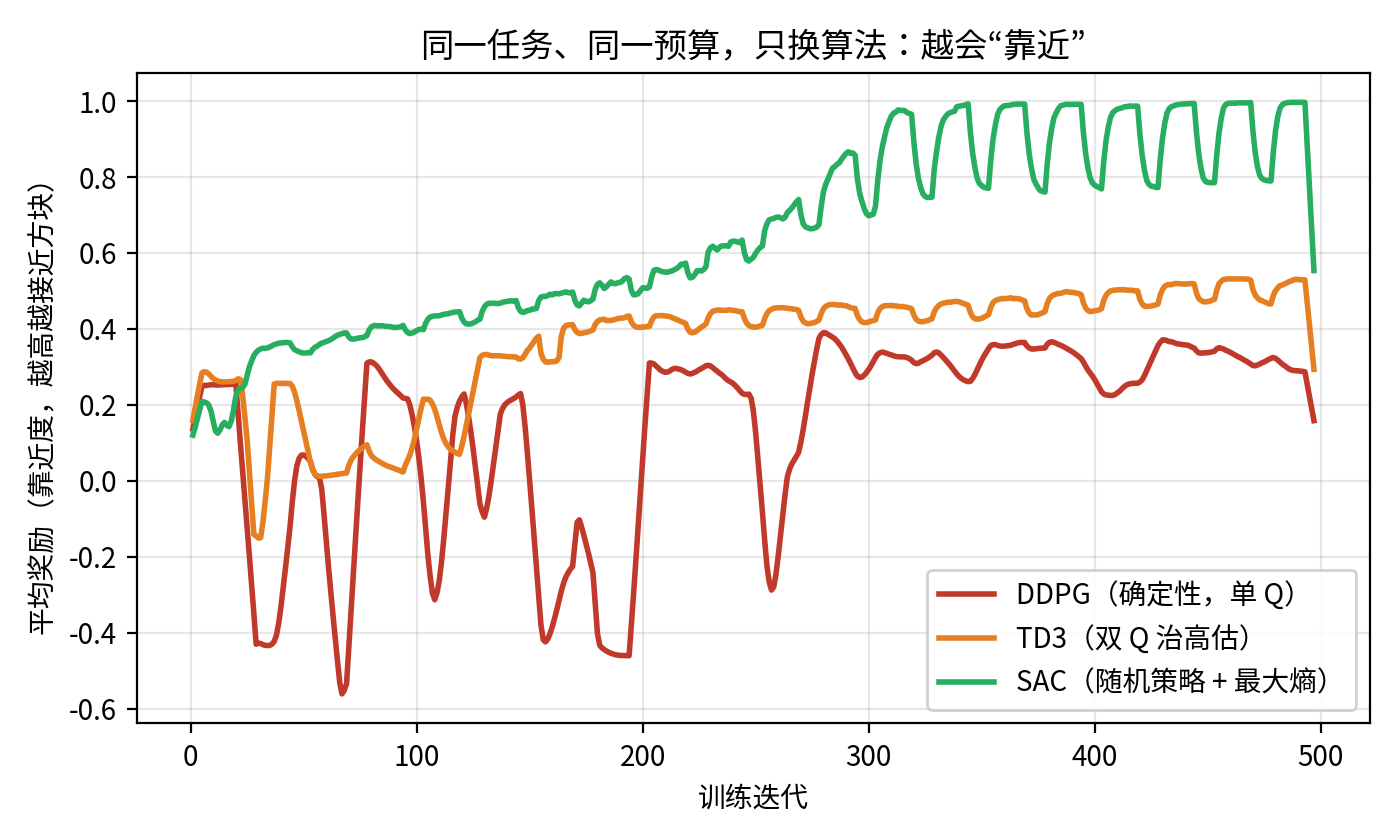
\includegraphics[width=0.95\linewidth,height=\textheight,keepaspectratio]{../../assets/figures/lecture16/ref/fig-so101-ladder-reward.png}

}

\caption{同一任务、同一预算（500
次迭代），只换算法：DDPG（红）剧烈震荡卡在低位，TD3（橙）稳住并爬到更高，SAC（绿）稳步登顶。纵轴平均奖励是''靠近度''的代理------越高表示末端越接近方块}

\end{figure}%

但橙线爬到中途就\textbf{平了}，而且成功率\textbf{仍然是 0}------TD3
靠得更近，却始终没能真正够到方块。为什么治好了高估还是解不出？

因为 TD3 治的是 \textbf{Q 高估}，动的全是 Critic 那一侧；它的 Actor
依然是\textbf{确定性}的，探索依然靠\textbf{外加的那点高斯噪声}。而
ReachCube
真正卡住确定性策略的，不是高估，是\textbf{探索}------确定性策略加一点小噪声，在六维动作空间里翻来覆去就那么大范围，试探不到''精准够到方块''所需的那套动作。高估修好了，探索的天花板还在。

这恰恰说明：\textbf{双 Critic 不是万能药，它只解决它那一类问题。}
要跨过''够到''这道坎，得从探索本身下手------这是 SAC 的地盘。

\subsection{4.3 本节小结}\label{ux672cux8282ux5c0fux7ed3-3}

TD3 在 DDPG 上打三个补丁------双 Critic 取 min
治高估、延迟策略更新、目标策略平滑------把 DDPG
的剧烈震荡稳住，平均奖励爬得更高、离方块更近。但它的探索仍靠确定性策略外加噪声，成功率依旧是
0：治好了高估，治不了探索。跨过''够到''这道坎要换探索机制，交给 SAC。

\section{5
SAC：把探索变成一条原则}\label{sacux628aux63a2ux7d22ux53d8ux6210ux4e00ux6761ux539fux5219}

DDPG 和 TD3 都卡在同一个地方------确定性策略 +
外加噪声的探索太弱。SAC（Soft
Actor-Critic）从根上换掉这套探索：它让策略重新变成\textbf{随机}的，并且把''保持随机、多探索''写成训练目标的一部分。这一换，成功率从
0 一举冲到 0.99。

\subsection{5.1
最大熵：把''多探索''写进目标}\label{ux6700ux5927ux71b5ux628aux591aux63a2ux7d22ux5199ux8fdbux76eeux6807}

普通强化学习的目标只有一条：回报最大化。SAC
在它上面加了一项------\textbf{策略熵}最大化。熵衡量策略的随机程度：熵高，策略在多个动作间保持犹豫、乐于尝试；熵低，策略趋于孤注一掷。SAC
的目标变成''\textbf{在拿高回报的同时，尽量保持随机}''。

这一项的作用正是治探索：它不让策略过早地锁死到某一套确定动作上，而是逼着它持续在动作空间里铺开试探，直到真的找到''够到方块''的那条路。DDPG/TD3
是''选定一个动作 + 抖一抖''，SAC
是''维持一整个动作分布，且刻意不让它塌缩''------后者的探索强度不是一个量级。

\subsection{5.2 SAC
的四个零件}\label{sac-ux7684ux56dbux4e2aux96f6ux4ef6}

把 SAC 拆开，是四个零件（对照 DDPG/TD3 看差异）：

\begin{enumerate}
\def\labelenumi{\arabic{enumi}.}
\tightlist
\item
  \textbf{随机策略（挤压高斯 Actor）}：Actor
  不再输出一个确定动作，而是输出一个高斯分布的均值和标准差，动作从中采样、再用
  \texttt{tanh} 压进合法区间。有了分布，才谈得上熵。
\item
  \textbf{最大熵目标}：回报项里减去一个''熵的代价''，等价于奖励策略保持随机（上一小节）。
\item
  \textbf{自动温度
  \(\alpha\)}：熵这一项占多大权重，用一个可学习的温度系数 \(\alpha\)
  自动调------训练自己找''探索够用又不过头''的平衡，不用手调。
\item
  \textbf{双 Critic 取 min}：治高估这条从 TD3 继承下来，SAC 也用两个
  Critic 取小。
\end{enumerate}

\begin{center}
\begin{tabular}{@{}>{\raggedright\arraybackslash}p{\dimexpr 0.1250\linewidth - 2\tabcolsep\relax} >{\raggedright\arraybackslash}p{\dimexpr 0.1562\linewidth - 2\tabcolsep\relax} >{\raggedright\arraybackslash}p{\dimexpr 0.1562\linewidth - 2\tabcolsep\relax} >{\raggedright\arraybackslash}p{\dimexpr 0.2812\linewidth - 2\tabcolsep\relax}@{}}
\toprule\noalign{}
零件 & DDPG & TD3 & SAC \\
\midrule\noalign{}
策略 & 确定性 & 确定性 & \textbf{随机（高斯采样）} \\
探索 & 外加噪声 & 外加噪声 & \textbf{最大熵内生} \\
温度 \(\alpha\) & 无 & 无 & \textbf{自动调} \\
Critic & 单个 & 双 min & 双 min \\
\bottomrule\noalign{}
\end{tabular}
\end{center}

看这张表就清楚：SAC = TD3 的双 Critic + 一套全新的''随机策略 + 最大熵 +
自动温度''探索机制。前三级在 Critic 那侧修修补补，SAC
终于动了\textbf{策略}这一侧。

\subsection{5.3 破局：成功率从 0 到
0.99}\label{ux7834ux5c40ux6210ux529fux7387ux4ece-0-ux5230-0.99}

回到章首那张对照图的绿线：SAC 的平均奖励一路稳步登顶，远超 DDPG 和
TD3。更重要的是成功率------它是这条阶梯上\textbf{第一个真正把方块够到}的算法。

不过有个细节值得讲：SAC
需要\textbf{足够的训练时间}才破局。前两百次迭代它也只是零星成功，直到经验攒够、策略在熵的驱动下把动作空间探得足够透，成功率才在第
280 次迭代附近\textbf{一举}从接近 0 爬到 0.99：

\begin{figure}[H]

{\centering 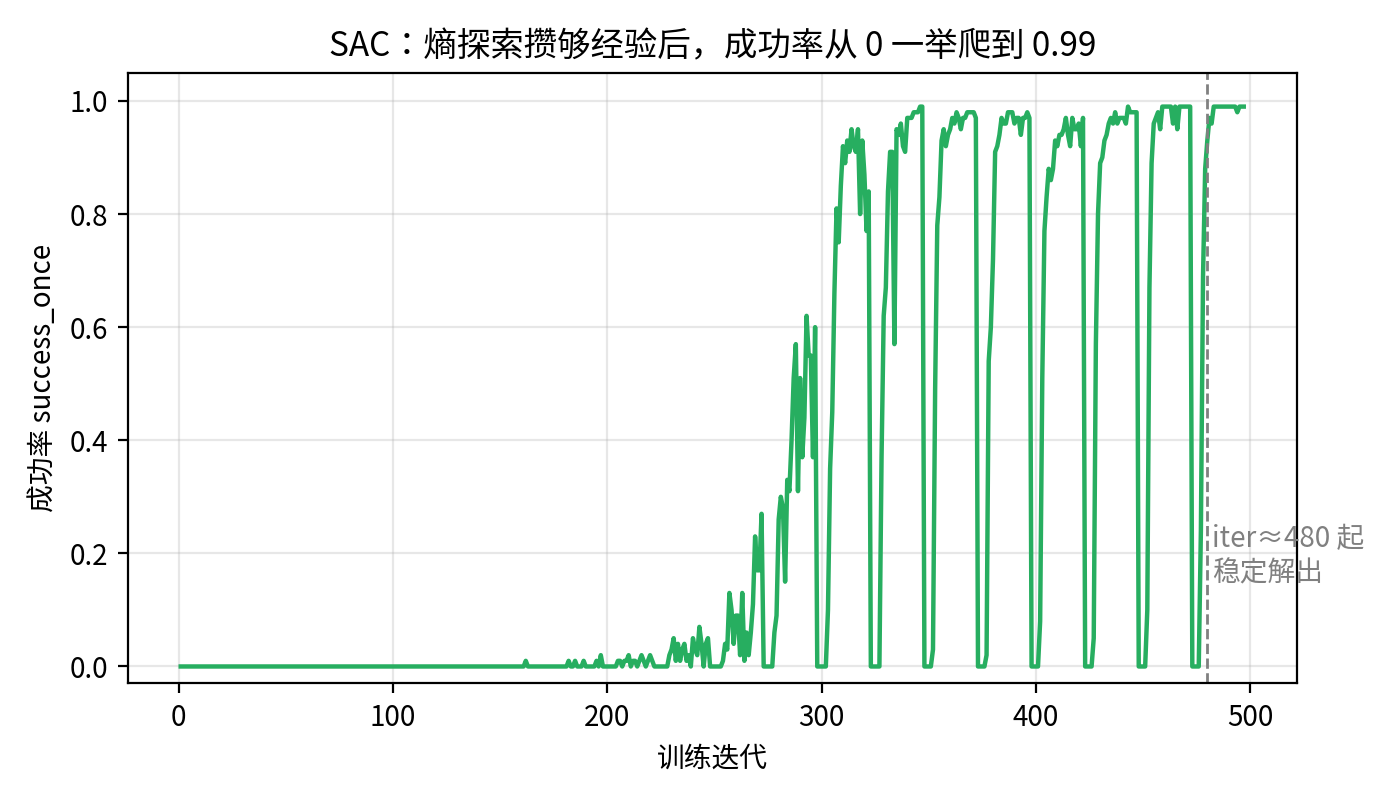
\includegraphics[width=0.9\linewidth,height=\textheight,keepaspectratio]{../../assets/figures/lecture16/ref/fig-sac-breakthrough.png}

}

\caption{SAC 的成功率曲线：前 200 多次迭代靠熵探索默默攒经验、成功率贴着
0；iter\(\approx 280\) 起一举冲到 0.99，但此后仍在 0 与 0.99
之间反复掉落，直到 iter\(\approx 480\) 才稳定解出}

\end{figure}%

这条''憋很久再突然起飞''的曲线本身就是探索型学习的典型形态------不是线性进步，是量变到质变。但要看清后半段：冲上去之后成功率还会成片地掉回
0，来回拉锯近两百次迭代才真正站稳。\textbf{``第一次做成''和''稳定做成''之间隔着的这段，才是真机上最耗时间的部分。}

\subsection{5.4
一张图看懂整条阶梯的两层道理}\label{ux4e00ux5f20ux56feux770bux61c2ux6574ux6761ux9636ux68afux7684ux4e24ux5c42ux9053ux7406}

把四级放在一起，成功率是这样一个阶梯：

\begin{figure}[H]

{\centering 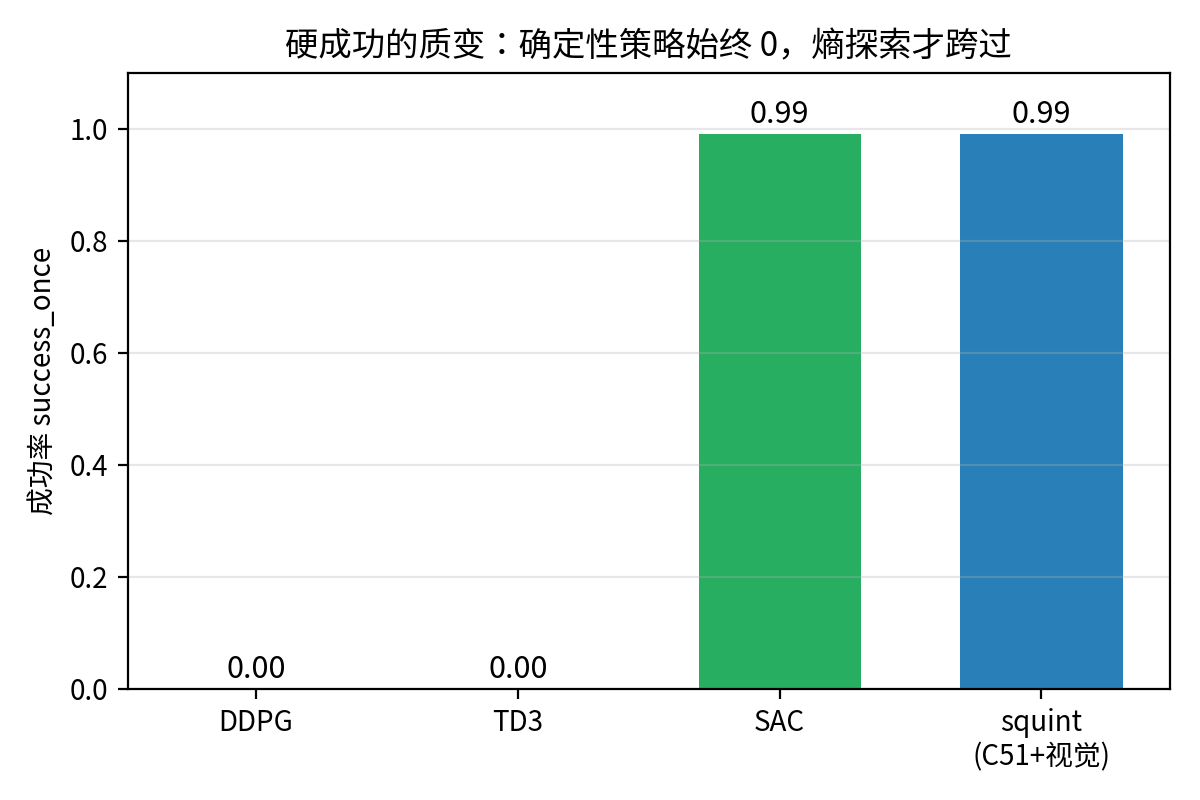
\includegraphics[width=0.8\linewidth,height=\textheight,keepaspectratio]{../../assets/figures/lecture16/ref/fig-so101-ladder-success.png}

}

\caption{成功率阶梯：DDPG 与 TD3 始终 0，SAC 冲到
0.99，squint（下一节）同样 0.99
但从像素学会。确定性策略越靠越近却始终跨不过''成功''那道坎，熵探索才跨过去}

\end{figure}%

把这张成功率图和前面那张靠近度（奖励）图叠着看，能读出\textbf{两层不同的道理}，这也是这条阶梯最想让你记住的：

\begin{itemize}
\tightlist
\item
  \textbf{靠近度是单调的}：DDPG \textless{} TD3 \textless{}
  SAC，每一级都比上一级更会靠近方块。从这个角度看，每一级的改进都实实在在有效------TD3
  的双 Critic、SAC 的熵探索，都让策略离目标更近了。
\item
  \textbf{硬成功是有质变的}：DDPG 和 TD3 无论靠得多近，成功率都死死是
  0；只有 SAC
  跨过了''够到''那道坎。这说明\textbf{``离得更近''和''真正解决''是两回事}------把方块从''差一点''推到''够到''，靠的不是把距离一点点磨小（那样
  DDPG/TD3
  迟早也能到），而是探索方式的\textbf{质变}：确定性策略的探索有天花板，最大熵才能顶破它。
\end{itemize}

一句话：\textbf{在这个任务上，探索------而不是高估、也不是网络容量------才是那把决定''解不解得出''的钥匙。}

\subsection{5.5 本节小结}\label{ux672cux8282ux5c0fux7ed3-4}

SAC 把探索从''外加噪声''换成''最大熵''这条原则：随机策略 + 熵最大化 +
自动温度，逼着策略持续铺开试探，直到真正找到够到方块的动作。它是这条阶梯上第一个把成功率做上去的算法（0→0.99，且需攒够时间才在
iter\(\approx 480\)
破局）。叠看靠近度与成功率两张图，读出两层道理：靠近度逐级单调、每级改进都有效，但硬成功有质变，探索才是解出任务的钥匙。SAC
用的还是标量 Critic + 均方误差，样本效率仍有提升空间------这是 squint
的切入点。

\section{6
squint：从像素学会，顺手把数据也生成了}\label{squintux4eceux50cfux7d20ux5b66ux4f1aux987aux624bux628aux6570ux636eux4e5fux751fux6210ux4e86}

到 SAC 为止，机械臂已经能从\textbf{关节状态}够到方块了。但真机上部署 VLA
时，策略看到的是\textbf{相机图像}，不是上帝视角的关节读数。第 6 级
squint 把两件事一起解决：一是把输入从状态换成\textbf{像素}，二是把
Critic
从标量升级成\textbf{分布式}，让它在更难的视觉输入上依然又快又稳地学会------顺带，它训好的策略还能直接拿去\textbf{生成
VLA 课要的仿真数据集}。

\subsection{6.1 分布式
Critic（C51）：不估一个数，估一整条分布}\label{ux5206ux5e03ux5f0f-criticc51ux4e0dux4f30ux4e00ux4e2aux6570ux4f30ux4e00ux6574ux6761ux5206ux5e03}

前几级的 Critic 都是估\textbf{一个}标量 Q 值。squint 用的 C51 分布式
Critic
换了个思路：不估''预期回报是多少''，而是估''回报\textbf{落在各个取值上的概率分布}长什么样''。

直觉上，回报本身是有不确定性的------同一个状态动作，运气好回报高、运气差回报低。硬压成一个平均数会丢掉这层结构；让网络直接去学整条分布，训练信号更丰富、梯度更稳，\textbf{样本效率显著更高}。这就是为什么
squint 在更难的视觉输入上，反而能学得比标量 SAC 更快更稳。

一个旁证：把标量 SAC 直接搬到视觉输入上，成功率只有百分之几；换成 C51
分布式 Critic，同样的视觉输入能到 0.99。\textbf{分布式 Critic
是视觉这一档样本效率的钥匙}，正如熵探索是''解不解得出''的钥匙。

\subsection{6.2 从 16
像素学会操作}\label{ux4ece-16-ux50cfux7d20ux5b66ux4f1aux64cdux4f5c}

squint 的另一半是视觉编码器：把相机图像降到很小的分辨率（16×16
像素）过一个小 CNN 编码，再接上和 SAC
同款的随机策略。别看分辨率低，配上分布式 Critic
和大规模并行采样，它照样能从零学会 ReachCube，成功率
0.99------而且这次策略看的是\textbf{像素}，离真机部署的输入形态更近了一步。

代码上 squint 就是把 SAC 的标量双 Critic 换成
\texttt{C51TwinQ}、前面接一个 CNN
编码器，其余训练骨架不变（\texttt{train\_v6\_squint.py}，同样自包含一个文件）。

\subsection{6.3
顺手生成数据：闭合整条数据链}\label{ux987aux624bux751fux6210ux6570ux636eux95edux5408ux6574ux6761ux6570ux636eux94fe}

squint
训好的策略不只是这条教学阶梯的终点，它还有一个下游用途，把这一讲和 VLA
课接成一个闭环。

回到第 3 章开头那句话：\textbf{RL 训练用的环境，和 VLA
课评测、复现数据用的是同一个环境}。既然 squint
已经能在这个环境里稳定够到方块，那就让它多跑几百条成功轨迹、把每条轨迹换个贴近真机的外观（黑臂、白底）重渲一遍，转成
VLA 课要的标准数据集格式------一套 VLA
微调数据就这么''顺手''生成出来了。这条流水线独立收在模块的
\texttt{datagen/}
文件夹里：策略跑轨迹、换外观重渲、转成数据集，一条命令串起来。

这里正好回收 VLA 课埋下的那个伏笔：\textbf{第9讲、第12讲里，你们用来微调
VLA
的那批仿真数据，当时只说''是用视觉强化学习从零生成的''、没有展开。现在你自己走到了这一步------从零训一个视觉
RL
策略、让它生成数据------也就真正理解了那批数据是怎么来的，甚至能自己复现一份。}
一门课里''先给你用、最后教你造''的完整闭环，到这里合上了。

\subsection{6.4 本节小结}\label{ux672cux8282ux5c0fux7ed3-5}

squint 在 SAC 的随机策略基础上做两件事：把标量 Critic 换成 C51 分布式
Critic（估回报的整条分布而非一个均值，样本效率显著提高，是视觉这一档能学会的钥匙），把输入从关节状态换成
16 像素视觉（贴近真机部署形态）。它从零学会 ReachCube 成功率
0.99，训好的策略再顺手 rollout + 换色生成 VLA 微调数据集，回收了第9/12
讲''数据是视觉 RL 生成''的伏笔，把这一讲和 VLA
课闭成一个''先用后造''的完整数据闭环。

\section{7 同一个 G1，换 off-policy 再走一遍：15
分钟学会走路}\label{ux540cux4e00ux4e2a-g1ux6362-off-policy-ux518dux8d70ux4e00ux904d15-ux5206ux949fux5b66ux4f1aux8d70ux8def}

我们在 SO-101 上从零爬完了 off-policy 阶梯------从表格 Q
一路到能从像素学会的 squint。最后把镜头拉回第14讲的老地方 G1
行走，看看业界怎么把同一套 off-policy
规模化：它真能在大规模并行仿真里顶替 on-policy 吗？2025
年恰好有一对工作把这件事做成了标杆。

\subsection{7.1 FastTD3 与 FastSAC：把 off-policy
搬进大规模并行仿真}\label{fasttd3-ux4e0e-fastsacux628a-off-policy-ux642cux8fdbux5927ux89c4ux6a21ux5e76ux884cux4effux771f}

off-policy
算法（SAC、TD3）在机器人学界长期被认为''样本效率高但难伺候''，主流的大规模并行仿真训练（第14讲那套
4096 环境 + PPO）一直是 on-policy 的天下。Amazon FAR 团队的
\textbf{FastTD3}
打破了这个格局：他们发现只要几处关键设计调对，off-policy
完全能在数千个并行环境的规模下稳定训练，而且\textbf{更快}。配方简单得出奇：

\begin{itemize}
\tightlist
\item
  \textbf{并行采样进同一个 replay
  buffer}：几千个环境同时交互，所有转移汇入一个大池子------并行仿真的吞吐和经验复用的效率第一次叠加在一起。
\item
  \textbf{大 batch 更新}：每次从池子里采上万条转移做一步梯度，充分喂饱
  GPU。
\item
  \textbf{高更新采样比（UTD）}：每采一步环境交互，做多次梯度更新------on-policy
  做不到的''一份数据榨多次''，off-policy 的看家本领。
\item
  \textbf{精心调校的稳定性配件}：双 Q 取小、目标网络软更新等（2.5
  节说过，这些是 off-policy 的必要开销）。
\end{itemize}

FastTD3 在 HumanoidBench 等人形基准上把训练时间压到单张 A100
上三小时以内，并把学到的策略部署上了 Booster T1
全尺寸人形真机；\textbf{FastSAC} 是同一配方套在 SAC 上的版本。

\subsection{7.2 结果：G1 行走，单卡 15
分钟}\label{ux7ed3ux679cg1-ux884cux8d70ux5355ux5361-15-ux5206ux949f}

后续工作《Learning Sim-to-Real Humanoid Locomotion in 15
Minutes》把这套配方推到了极致：在单张 RTX 4090 上，\textbf{15
分钟}训出能通过 sim-to-real 部署到 Unitree G1 和 Booster T1
真机的行走策略------训练时还开着强域随机化（随机动力学、粗糙地形、外力推搡）。下图取自该论文，上排是训好的策略部署在真机上的照片，下排是训练曲线。

\begin{figure}[H]

{\centering 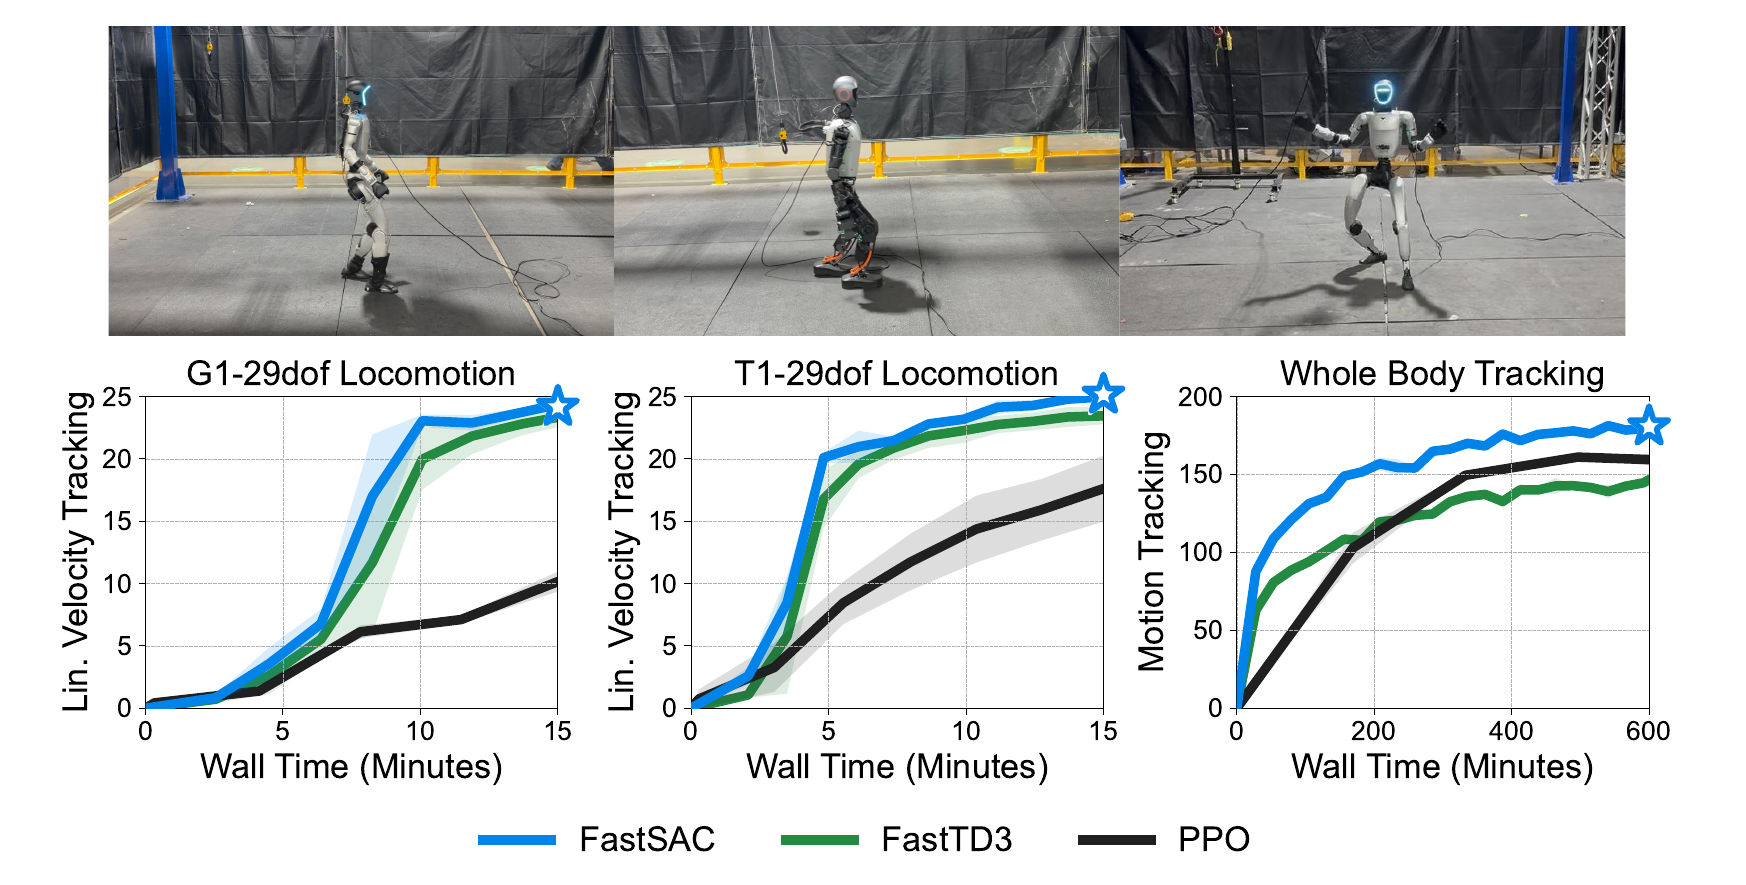
\includegraphics[width=0.92\linewidth,height=\textheight,keepaspectratio]{../../assets/figures/lecture16/ref/fig163-fastsac-15min-summary.png}

}

\caption{FastSAC/FastTD3 与 PPO 在 G1、T1
行走和全身动作跟踪上的墙钟时间对比，上排为 sim-to-real 部署到真机的画面}

\end{figure}%

曲线的读法：横轴是\textbf{墙钟时间}（不是环境步数），纵轴是速度跟随任务的回报。左、中两张图里，蓝线（FastSAC）和绿线（FastTD3）在
10 分钟上下就冲到平台期，而黑线（PPO）在同一个 15
分钟窗口内还在半山腰。右图是更难的全身动作跟踪（和第14讲 BeyondMimic
同类任务），时间尺度拉长到 600 分钟------这里要看仔细：\textbf{只有
FastSAC 全程领先}，FastTD3 前期虽快，约 350 分钟后被 PPO
反超、最终收在它下面。所以 off-policy
的墙钟优势在长时间尺度上并非无条件成立，换个算法就可能翻盘。

\begin{quote}
备注：这是\textbf{同一块 GPU 上的墙钟对比}，不是''PPO
学不会''------给足时间 PPO 也能到平台。off-policy 每一步更新更重（大
batch、多次梯度），但样本复用让它总体上快得多。另外论文用了\textbf{极简奖励函数}------off-policy
对奖励设计的品味和 on-policy
不完全一样，把第14讲的奖励原样搬过来不一定最优。
\end{quote}

这个结果和第14讲形成了一组干净的对照：\textbf{同一台
G1、同一类行走任务}，第14讲的 PPO 靠 4096 个环境堆出上亿步交互，这里的
FastSAC
靠''每条经验反复用''把墙钟压缩到一刻钟。第14讲埋的''为什么真机要换
off-policy''，在仿真里就已经初见分晓。

\subsection{7.3 动手实验：给 G1
行走加第四个版本}\label{ux52a8ux624bux5b9eux9a8cux7ed9-g1-ux884cux8d70ux52a0ux7b2cux56dbux4e2aux7248ux672c}

第14讲的 \texttt{1\_1\_g1\_walk\_rl}
模块里躺着三个训练脚本：\texttt{train\_v1\_reinforce.py}、\texttt{train\_v2\_a2c.py}、\texttt{train\_v3\_ppo.py}------同一个任务，算法由简到繁。SO-101
阶梯之外再补一个动手实验：给第14讲这条 G1
阶梯加\textbf{第四级}------off-policy 的 SAC
版本，环境、奖励、模型骨架全部复用，只换算法。

实验设计如下：

\begin{itemize}
\tightlist
\item
  \textbf{任务与环境}：与第14讲完全相同的 mjlab G1
  平地速度跟随环境（\texttt{G1WalkEnv}），不改任何奖励项------保证对照干净。
\item
  \textbf{代码结构}：和 v1 到 v3 一样的 Lightning
  四件套。最有教学价值的差异在数据层：前三个版本的 \texttt{Dataset}
  每轮\textbf{在线采一段新 rollout}，SAC 版本换成
  \textbf{\texttt{ReplayBufferDataset}}------转移存进池子、随机抽样训练。\textbf{on-policy
  和 off-policy 的全部区别，在数据这一层直接看得见。}
\item
  \textbf{训练配方}：取 FastSAC
  配方中对课堂有意义的三件------并行环境采样进同一个 buffer、大
  batch、高 UTD；distributional critic 等纯提速细节不进这个 G1
  版本，保持代码能一口气读懂。
\item
  \textbf{对照口径}：两张曲线图。第一张按\textbf{环境步数}对齐------预期
  off-policy
  在早期样本效率上显著占优，这是''每条经验反复用''的直接兑现；第二张按\textbf{墙钟时间}对齐------诚实展示
  off-policy 每步更新更贵的另一面。最后配 rollout 视频对照步态质量。
\end{itemize}

这套实验已经落进课程代码仓：\texttt{1\_1\_g1\_walk\_rl} 模块新增
\texttt{train\_v4\_sac.py}，与前三个版本并排摆放，对照曲线与 rollout
视频在同模块的 \texttt{result/} 里。下面按结果读图。

\textbf{先回答最要紧的问题：它会不会走？} 会。确定性评测（256 个环境各跑
300 步）摔倒率约
1\%，抽帧里能看到真实的迈步------不是站桩，也不是高频抽搐。但平均 reward
停在 0.026，只有 v3 PPO（0.097）的三分之一不到。

\begin{figure}[H]

{\centering 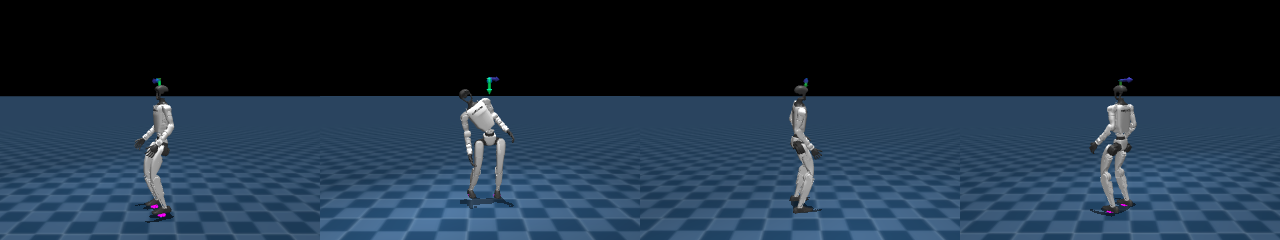
\includegraphics[width=0.92\linewidth,height=\textheight,keepaspectratio]{../../assets/figures/lecture16/ref/fig-v4-sac-strip.png}

}

\caption{SAC 版本的 rollout 抽帧，G1 在速度指令下持续行走、全程保持直立}

\end{figure}%

\textbf{再看两张对照曲线。} 第一张按环境步数对齐：SAC 大约 2 到 7M
步就爬到 \(10^{-2}\) 量级的 reward 并稳定行走；而 PPO 的第一个存档点在
20M 步（当时已到 0.064）。要小心的是，20M 步之前 PPO
没有存档，两条曲线的''交叉点''并没有实测------所以这张图只支持一个定性结论：\textbf{off-policy
在起步阶段确实更省交互}，不支持''省了多少倍''这样的定量说法。第二张按墙钟对齐：SAC
全程约 15 分钟，PPO 约 100 分钟------7.2 节里论文的''15
分钟''，在我们自己的环境里复现出了同一个量级。

\begin{figure}[H]

{\centering 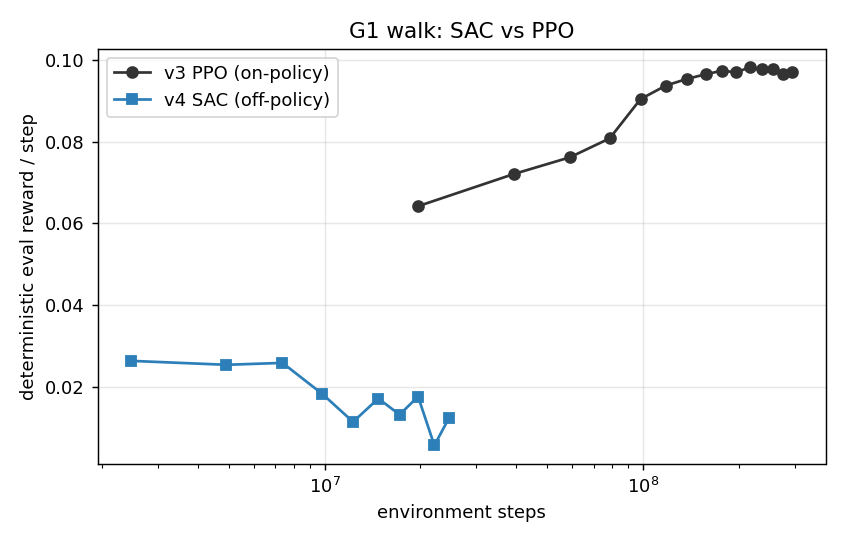
\includegraphics[width=0.88\linewidth,height=\textheight,keepaspectratio]{../../assets/figures/lecture16/ref/fig-v4-sac-envsteps.png}

}

\caption{按环境步数对齐的 reward 曲线（横轴对数刻度）：SAC 在 2--7M
步就稳定在 \(10^{-2}\) 量级，整段曲线都落在图的左侧；PPO
的第一个存档点要到 20M 步，此后一路爬到 0.097 的平台}

\end{figure}%

\begin{figure}[H]

{\centering 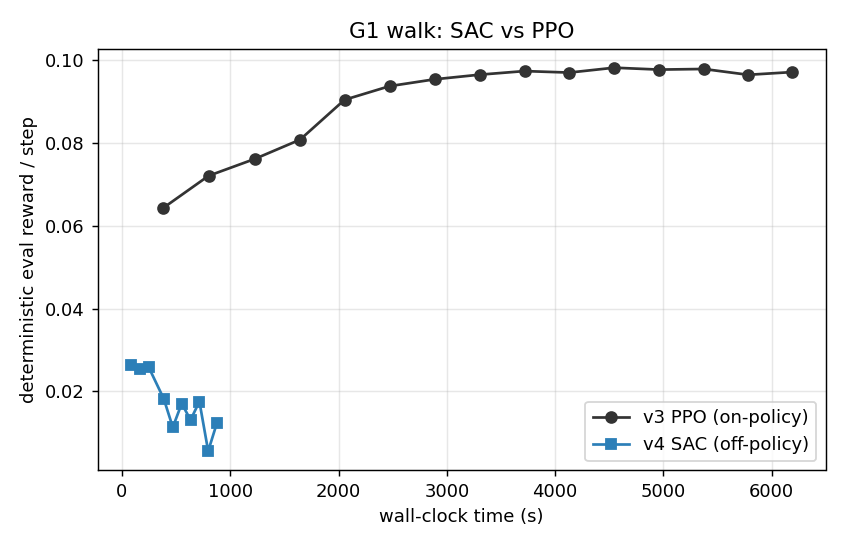
\includegraphics[width=0.88\linewidth,height=\textheight,keepaspectratio]{../../assets/figures/lecture16/ref/fig-v4-sac-walltime.png}

}

\caption{按墙钟时间对齐的 reward 曲线，SAC 全程约 15 分钟、PPO 约 100
分钟}

\end{figure}%

\begin{center}
\begin{tabular}{@{}>{\raggedright\arraybackslash}p{\dimexpr 0.0843\linewidth - 2\tabcolsep\relax} >{\raggedright\arraybackslash}p{\dimexpr 0.2568\linewidth - 2\tabcolsep\relax} >{\raggedright\arraybackslash}p{\dimexpr 0.1203\linewidth - 2\tabcolsep\relax} >{\raggedright\arraybackslash}p{\dimexpr 0.1108\linewidth - 2\tabcolsep\relax} >{\raggedright\arraybackslash}p{\dimexpr 0.2482\linewidth - 2\tabcolsep\relax} >{\raggedright\arraybackslash}p{\dimexpr 0.1795\linewidth - 2\tabcolsep\relax}@{}}
\toprule\noalign{}
版本 & 算法 & reward & 摔倒率 & 到最佳档的交互量 & 全程墙钟 \\
\midrule\noalign{}
v3 & PPO（on-policy） & 0.097 & 0\% & 295M 步 & 约 100 分钟 \\
v4 & SAC（off-policy） & 0.026 & 约 1\% & 7.4M 步 & 约 15 分钟 \\
\bottomrule\noalign{}
\end{tabular}
\end{center}

\textbf{为什么没追上 PPO 的平台？} 两个原因，7.2
节的备注其实都预告过：这套奖励本来是给 PPO 调的，off-policy
的品味不一样；而且课堂版刻意只保留 SAC 最核心的零件，FastSAC 里的 n-step
回报、分布式 critic
这些提速件都没上------它们正是论文里绝对性能的来源。所以这张对照图的正确读法不是''SAC
不行''，而是：\textbf{样本效率与绝对性能是一对要靠配方去调和的矛盾}------起步省交互是
off-policy 结构性的优势，绝对高度则要靠完整配方去挣。

\textbf{跑通之前先踩了三个坑}，每一个都是第 5
节讲过的零件在真实训练里的反面教材，值得记下来：

\begin{enumerate}
\def\labelenumi{\arabic{enumi}.}
\tightlist
\item
  \textbf{奖励尺度}。G1 每步 reward 只有 0.05 上下，直接进 SAC
  的目标会被熵项整个淹没------actor
  优化的全是''保持随机''，机器人永远站着不动。把 reward
  放大十倍之后，任务信号才压得过熵。回头看 5.1 节的目标函数：reward
  和熵是相加的两项，谁的量级大谁说了算。
\item
  \textbf{温度失守}。自动温度（5.2 节的第四个零件）会自己往下调
  \(\alpha\)，训到后期 \(\alpha\) 掉到 0.01
  附近，熵正则实际上消失，策略开始把动作越顶越大、步态反而退化。解法是给
  \(\alpha\) 设一个 0.1
  的下限------自动温度照常工作，但不许它把探索完全关掉。
\item
  \textbf{动作幅度}。tanh 挤压的输出上限一开始设成
  3.0，策略学出灾难性的大幅甩动；收回 1.0（这个环境的动作本来就是 1
  上下的量级）才回到正常步态。
\end{enumerate}

三个坑合起来是一句话：\textbf{off-policy
的稳定性从来不是白来的}------同一份代码，几个数值不对就完全不收敛。这也为第
8 节埋下伏笔：真机方案要在 SAC
之上再垫示教、干预这么多层保险，正是因为它在真机上连''重训一次试试''的机会都没有。

\subsection{7.4 本节小结}\label{ux672cux8282ux5c0fux7ed3-6}

本节用 FastTD3/FastSAC 回答了''off-policy
行不行''：不但行，在大规模并行仿真里还更快------单卡 15 分钟训出能上 G1
真机的行走策略，核心配方是并行采样进同一个 replay buffer、大 batch、高
UTD。我们自己的第四版动手实验印证了这条路的两面：起步省交互、墙钟压到一刻钟是结构性的，绝对高度则要靠完整配方去挣。它的局限也要看清：这仍然是\textbf{仿真里}的胜利，奖励函数是白拿的、复位是免费的、探索撞坏了按
R 重来。下一节把这三张''仿真特权卡''全部收走，看看真机上还缺什么。

\section{8 真机压轴：HIL-SERL 让 SO-101
学会接触型任务}\label{ux771fux673aux538bux8f74hil-serl-ux8ba9-so-101-ux5b66ux4f1aux63a5ux89e6ux578bux4efbux52a1}

阶梯爬到
squint，我们已经能在仿真里从零学会一个操作任务了。但那仍是\textbf{仿真里}的胜利------奖励是白拿的、复位是免费的、探索撞坏了按
R
重来。这一节把这三张''仿真特权卡''全部收走，看看真机上还缺什么，再用一整套工程答案把它补齐。好消息是不用从头造轮子：这套答案叫
\textbf{HIL-SERL}，而且已经被 LeRobot 官方移植到
SO-100/SO-101------第9讲采数据用的那套主从臂，现在原封不动就能变成一套真机强化学习装备。所以这一节采取''\textbf{概念一件、操作一件}''的走法：每讲清
HIL-SERL 的一个部件，紧接着就给出它在 LeRobot 里对应的那一步命令。

\subsection{8.1 把 SAC
搬上真机：四道坎}\label{ux628a-sac-ux642cux4e0aux771fux673aux56dbux9053ux574e}

把前面 SO-101 阶梯上的 SAC 直接搬上一台真实机械臂，会立刻撞上四道坎：

\begin{enumerate}
\def\labelenumi{\arabic{enumi}.}
\tightlist
\item
  \textbf{奖励谁来发？} 仿真器里 reward
  是一行代码，因为仿真器知道每个物体的真实位姿。真机上没有上帝视角------``插头插进去了没有''，只有相机看得见。
\item
  \textbf{谁来复位？} 仿真里回合结束一键
  reset。真机上方块掉在地上不会自己飞回桌面。
\item
  \textbf{探索会闯祸。}
  随机初始化的策略在真机上乱抡，轻则任务毫无进展，重则撞坏夹爪和工件。
\item
  \textbf{样本贵上加贵。} 第 1
  节算过的账，在接触型任务上更严苛------插拔、对位这类任务容错以毫米计，瞎探索几乎撞不出成功，稀疏奖励长期是零，学习根本启动不了。
\end{enumerate}

\textbf{HIL-SERL}（Human-in-the-Loop Sample-Efficient Reinforcement
Learning，UC Berkeley）就是针对这四道坎给出的一整套工程答案，发表于
Science Robotics。它不发明新算法，而是把一条成熟的 off-policy
血缘链带上真机，再补上''人''这个要素。

\subsection{8.2 一条血缘链：SAC 到
HIL-SERL}\label{ux4e00ux6761ux8840ux7f18ux94fesac-ux5230-hil-serl}

HIL-SERL
不是凭空出现的，它是伯克利同一条线上四步演进的终点，每一步只解决一个问题：

\begin{center}
\begin{tabular}{@{}>{\raggedright\arraybackslash}p{\dimexpr 0.1390\linewidth - 2\tabcolsep\relax} >{\raggedright\arraybackslash}p{\dimexpr 0.0765\linewidth - 2\tabcolsep\relax} >{\raggedright\arraybackslash}p{\dimexpr 0.7846\linewidth - 2\tabcolsep\relax}@{}}
\toprule\noalign{}
工作 & 年份 & 在前一步上补了什么 \\
\midrule\noalign{}
SAC & 2018 & 连续动作 off-policy 的算法底座（第 5 节） \\
RLPD & 2023 & \textbf{先验数据进池子}：每个 batch 一半采自在线经验、一半采自离线示教；配上高 UTD 和 LayerNorm 稳住 critic \\
SERL & 2024 & \textbf{软件套件}：actor 与 learner 分进程解耦、阻抗控制器保护硬件、免复位训练支持 \\
HIL-SERL & 2024 & \textbf{人在环}：训练中人工干预 + 视觉奖励分类器，通吃接触型任务 \\
\bottomrule\noalign{}
\end{tabular}
\end{center}

链条中间的 \textbf{RLPD}（RL with Prior Data）值得多说两句，因为
HIL-SERL 的 learner 跑的就是它。它对 SAC
只做三处改动，每处都对着一个真机痛点：

\begin{itemize}
\tightlist
\item
  \textbf{对半采样}：每个训练 batch
  一半抽自在线经验池、一半抽自示教池。比例焊死在五五开是刻意的------全吃示教会过拟合到''学得像''（那是模仿学习的地界），全吃在线经验又回到冷启动的老问题；对半保证每一步更新既有''成功长什么样''的锚，又有''我自己刚犯的错''的新鲜教训。
\item
  \textbf{高 UTD}：每采一步做多次梯度更新（2.5 节说的 UTD
  杠杆），把真机上贵得要命的每条转移榨干。
\item
  \textbf{critic 加 LayerNorm}：高 UTD 会放大死亡三角的风险，尤其是
  critic 对\textbf{没见过的动作}报出离谱高分、被 actor
  钻空子的问题；LayerNorm
  把网络输出的量级压住，是让''猛榨样本''不翻车的关键配平。
\end{itemize}

记住这条链的读法：\textbf{SAC 给能力，RLPD 给样本效率，SERL
给工程骨架，HIL-SERL 给真机落地的最后一公里。}

下面就把 HIL-SERL 拆成''四件套 + actor-learner
架构''逐个讲透------每讲完一件，紧接着给出它在 LeRobot SO-101
上对应的那一步操作。

\subsection{8.3
落到我们的硬件：角色分工与第一步------划安全边界}\label{ux843dux5230ux6211ux4eecux7684ux786cux4ef6ux89d2ux8272ux5206ux5de5ux4e0eux7b2cux4e00ux6b65ux5212ux5b89ux5168ux8fb9ux754c}

先把任务和硬件摆好。\textbf{任务}选接触型的入门款：\textbf{把方块推到目标区域}（push
cube to goal
region）。它具备接触任务的全部要素------推的力道和角度直接决定成败、视觉可判定成功------又足够短（5
到 10 秒一个回合），符合 HIL-SERL
的甜区。练顺之后可以升级到抓取-提起（pick and lift）。

\textbf{硬件分工}和第9讲遥操作采数据时一模一样，但角色变了：

\begin{itemize}
\tightlist
\item
  \textbf{follower 臂}：不再重放人的动作，而是作为 \textbf{RL actor
  的身体}，执行策略输出的动作、与环境真实交互。
\item
  \textbf{leader
  臂}：不再全程主导，而是作为\textbf{人的干预接口}------训练中它实时跟随
  follower 的姿态，人随时可以握住它接管几步（SO-101 leader
  的减速齿轮让''顺滑接管''成为可能），键盘 space
  键在''策略控制''和''人控制''之间切换。
\item
  \textbf{两路相机}（顶视 +
  腕视）：既是策略的眼睛，也是奖励分类器的裁判席。
\end{itemize}

动作空间有一个关键选择：\textbf{在末端执行器（EE）空间学，不在关节空间学}。策略输出的是末端的
x、y、z
位移增量，由逆运动学换算成关节目标。经验上，操作类任务在关节空间学 RL
要难得多------同样的任务换到 EE 空间往往才变得可学；而且 EE
空间里''划安全边界''直观得多。

这条 EE 边界正是 8.1
节第三道坎（探索会闯祸）的第一个工程回应，也是全流程的第一步操作。运行
\texttt{lerobot-find-joint-limits}，手动拖着 follower
把''完成任务需要的空间''扫一遍，脚本记录末端位置的最小、最大值：

\begin{Shaded}
\begin{Highlighting}[]
\ExtensionTok{lerobot{-}find{-}joint{-}limits} \DataTypeTok{\textbackslash{}}
  \AttributeTok{{-}{-}robot.type}\OperatorTok{=}\NormalTok{so101\_follower }\AttributeTok{{-}{-}robot.port}\OperatorTok{=}\NormalTok{/dev/ttyFollower }\DataTypeTok{\textbackslash{}}
  \AttributeTok{{-}{-}teleop.type}\OperatorTok{=}\NormalTok{so101\_leader }\AttributeTok{{-}{-}teleop.port}\OperatorTok{=}\NormalTok{/dev/ttyLeader}
\end{Highlighting}
\end{Shaded}

得到的边界写进配置的
\texttt{end\_effector\_bounds}。这一步同时回应了两件事：探索安全（策略出不了这个箱子），和学习难度（动作空间被压缩到任务相关的一小块）。

\subsection{8.4 第一件套 demo
buffer：示教打底，并采下示教}\label{ux7b2cux4e00ux4ef6ux5957-demo-bufferux793aux6559ux6253ux5e95ux5e76ux91c7ux4e0bux793aux6559}

\textbf{概念。} 训练开始前，先用遥操作采一批成功示教，装进一个独立的
\textbf{demo buffer}。这直接继承 RLPD：每个训练 batch
一半来自在线经验池、一半来自示教池------从第一次梯度更新起，网络就见过''成功长什么样''，不必从纯随机探索里大海捞针。这是对第四道坎（学习启动不了）的回答。

\textbf{操作。} 在 LeRobot 里，把配置文件 \texttt{mode} 设为
\texttt{"record"}，用 leader 遥操作采 \textbf{15 到 20
条成功示教}（论文里典型是 20 到 30 条）：

\begin{Shaded}
\begin{Highlighting}[]
\ExtensionTok{python} \AttributeTok{{-}m}\NormalTok{ lerobot.rl.gym\_manipulator }\AttributeTok{{-}{-}config\_path}\NormalTok{ env\_config\_so101.json}
\end{Highlighting}
\end{Shaded}

每条示教以人按下''成功''键结束（该回合最后一步记奖励 1）。数据落成标准
LeRobot 数据集------第9讲学的那套数据格式，在这里原样复用。

\subsection{8.5 第二件套
视觉奖励分类器：让相机当裁判，并把它训出来}\label{ux7b2cux4e8cux4ef6ux5957-ux89c6ux89c9ux5956ux52b1ux5206ux7c7bux5668ux8ba9ux76f8ux673aux5f53ux88c1ux5224ux5e76ux628aux5b83ux8badux51faux6765}

\textbf{概念。}
不手写奖励函数，也不让人逐帧打分，而是\textbf{把''成功了吗''学出来}：遥操作采集一批正样本（任务完成的画面）和负样本（没完成的画面）------论文的典型配比是约
200 正、1000 负，折合十来条轨迹、五分钟的事------训练一个基于 ResNet
的\textbf{二分类器}。训练时它盯着相机画面，输出 0/1
稀疏奖励，还顺带自动判断回合结束。这是对第一道坎（真机没有上帝视角）的回答。

\begin{quote}
备注：分类器也会被骗------机械臂挡住目标、光照变化都可能造成误判。假阳性尤其危险：策略会学会''摆拍''骗分。实践中靠提高判定阈值、追加难负样本来修，这也是下面训练分类器时要专门留心的点。
\end{quote}

\textbf{操作（一）：先框视觉关注区。} RL
直接从像素学习，对背景干扰极其敏感------光照变化、路过的人、工作区外的杂物都可能把学习带偏。上分类器之前，先用交互工具把每路相机的画面裁到任务核心区：

\begin{Shaded}
\begin{Highlighting}[]
\ExtensionTok{python} \AttributeTok{{-}m}\NormalTok{ lerobot.rl.crop\_dataset\_roi }\AttributeTok{{-}{-}repo{-}id} \OperatorTok{\textless{}}\NormalTok{你的示教数据集}\OperatorTok{\textgreater{}}
\end{Highlighting}
\end{Shaded}

框出的裁剪参数写进配置的 \texttt{crop\_params\_dict}，图像统一缩放到
\(128\times128\)。

\textbf{操作（二）：训练分类器。} 先把 \texttt{terminate\_on\_success}
设为 \texttt{false}
再采一批数据------回合在成功后\textbf{不}立即截断，让''成功状态''的画面多攒一些（正样本不足是分类器最常见的坑）；然后用
ResNet-10 底座训二分类器：

\begin{Shaded}
\begin{Highlighting}[]
\ExtensionTok{lerobot{-}train} \AttributeTok{{-}{-}config\_path}\NormalTok{ reward\_classifier\_train\_config.json}
\end{Highlighting}
\end{Shaded}

训完把模型路径写进配置的
\texttt{reward\_classifier.pretrained\_path}，判定阈值从 0.7
左右起调。上真机前先单独测一轮：故意摆几个''像成功但不是''的场面，看它会不会误判。

\subsection{8.6 第三、四件套
人工干预与自动复位}\label{ux7b2cux4e09ux56dbux4ef6ux5957-ux4ebaux5de5ux5e72ux9884ux4e0eux81eaux52a8ux590dux4f4d}

\textbf{人工干预（第三件套）。} 这是 HIL-SERL 名字里
``Human-in-the-Loop''
的本体。在线训练时人守在旁边，看到策略快要闯祸或卡死，\textbf{随时接管}遥操几步把机器人带回正轨，然后把控制权还给策略。关键在于干预数据的用法：\textbf{接管的那几步被当作高质量的
off-policy 转移，照常存进经验池参与训练}------2.1 节说过，off-policy
不挑数据来源，人的手就是另一个行为策略。

这与模仿学习里的 DAgger 家族形成一组重要对照：HG-DAgger
同样让人纠偏，但把纠偏数据拿去做\textbf{监督学习}------策略的上限被钉死在''学得像示范者''；HIL-SERL
把同样的数据交给\textbf{强化学习}------干预只是引路，策略最终按任务奖励自我优化，可以\textbf{超过}示范者（本章后面
8.8 与 HG-DAgger
的对照曲线会印证这一点）。这是对第三道坎（探索闯祸）的回答：人挡住最坏情况，策略保留自我提升空间。这一件套的操作接口就是
8.3 节说的 leader 臂 + space 键，具体命令并进下一节的在线训练里一起给。

\textbf{自动复位（第四件套）。} 回合结束后环境自动回到初始分布：SERL
提供了 forward-backward
双控制器的免复位方案（一个策略做任务、一个策略负责''拆回去''），SO-101
这类简单场景则用固定复位关节位加随机化初始姿态。人只负责偶尔把掉落的物体捡回工作区。这是对第二道坎（谁来复位）的回答。

\subsection{8.7 actor-learner
架构：拼成在线系统，并跑起来}\label{actor-learner-ux67b6ux6784ux62fcux6210ux5728ux7ebfux7cfbux7edfux5e76ux8dd1ux8d77ux6765}

四件套怎么拼成一个在线系统？下图是 HIL-SERL 论文的系统总览。

\begin{figure}[H]

{\centering 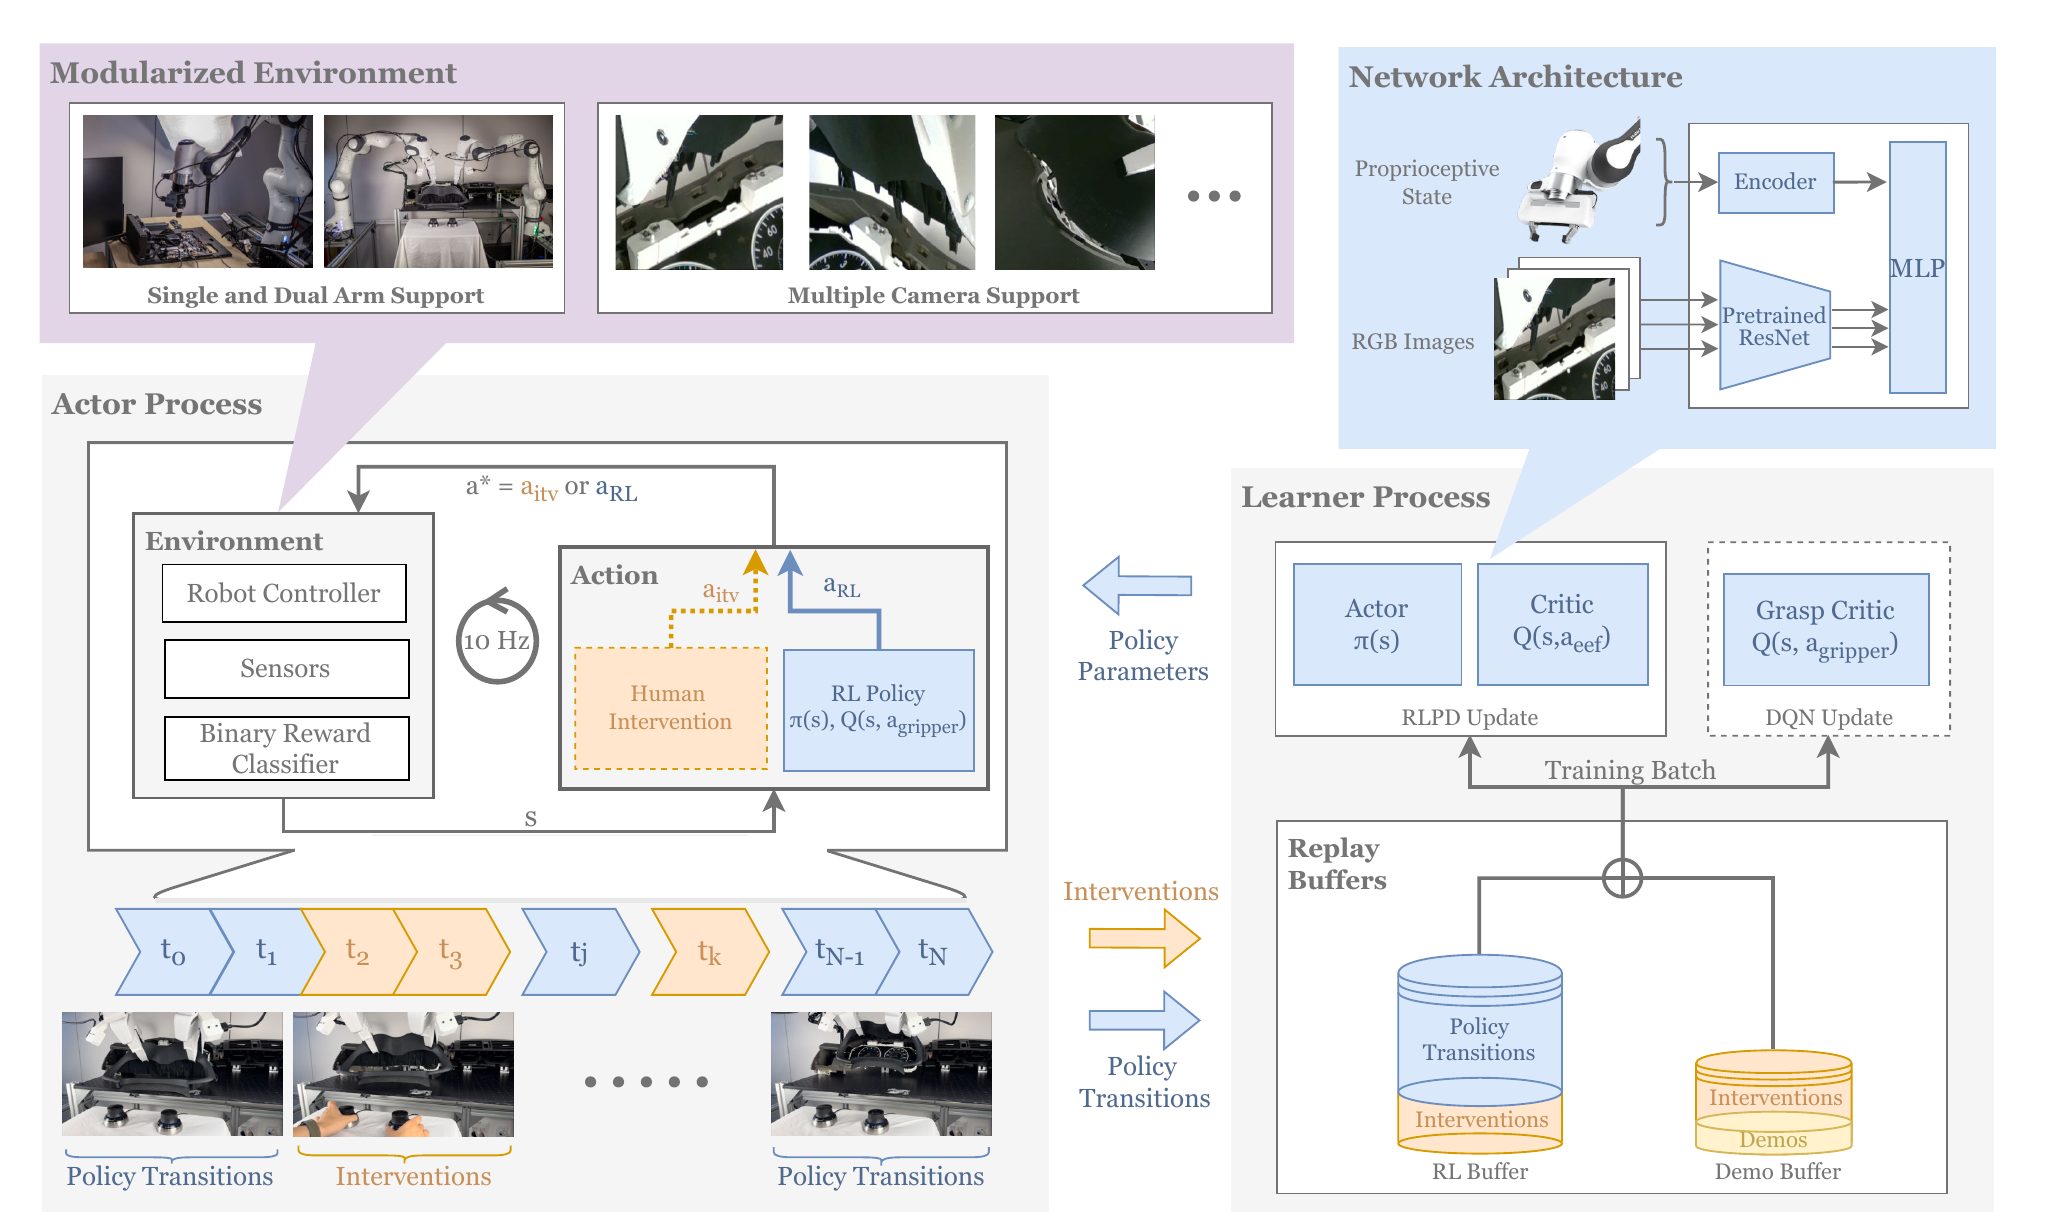
\includegraphics[width=1\linewidth,height=\textheight,keepaspectratio]{../../assets/figures/lecture16/ref/fig164-hilserl-architecture.png}

}

\caption{HIL-SERL 系统架构：actor
进程与环境实时交互并接受人工干预，learner 进程从双 replay buffer
采样更新，两者异步通信}

\end{figure}%

按数据流走一遍这张图：

\begin{itemize}
\tightlist
\item
  \textbf{左边 actor 进程}：以 10 Hz
  的固定节奏和环境交互。每一拍，环境给出观测 \(s\)（相机图像 +
  本体状态），动作要么来自 RL
  策略（\(a_{\mathrm{RL}}\)），要么来自人的干预（\(a_{\mathrm{itv}}\)，虚线路径）------谁在控制就听谁的。二值奖励分类器在环境侧充当裁判。时间轴上蓝色段是策略自主，黄色段是人接管。
\item
  \textbf{右下 replay buffers}：两个池子。RL buffer
  收所有在线转移（策略的和干预的），demo buffer
  存训练前采的示教；learner 每个 batch 从两池对半采样（RLPD 的规矩）。
\item
  \textbf{右边 learner 进程}：在 GPU 上闷头做梯度更新（actor 网络 +
  critic 网络），周期性把最新的策略参数推回 actor 进程。
\item
  \textbf{右上网络结构}：多路相机图像过同一个预训练 ResNet-10
  编码，与本体状态编码拼接后进 MLP。
\end{itemize}

actor 和 learner \textbf{异步解耦}是真机 RL
的硬需求，不是花活：真机控制必须踩着 10 Hz 的实时节拍，不能停下来等 GPU
算完一个 batch；反过来 GPU
也不该在机器人慢吞吞动作时闲着。分进程后两边各按各的节奏满负荷运转，这个设计在下面的
LeRobot 实现里原样保留。

LeRobot 把整套 HIL-SERL 封装成三块：环境侧的
\texttt{gym\_manipulator}（把真机包成 Gym
风格环境，串起奖励分类器、干预、安全边界等处理管线）、训练侧的
\texttt{lerobot.rl.learner} 与 \texttt{lerobot.rl.actor}
两个进程入口（正对上面架构图的两个进程），以及一份 JSON
配置文件贯穿全部环节------工程实现与 8.7 节那张论文架构图一一对应。

\textbf{操作：起两个进程做在线训练。}
边界、示教、分类器都就位后，两个终端分别拉起两个进程，人守在 leader
旁边：

\begin{Shaded}
\begin{Highlighting}[]
\ExtensionTok{python} \AttributeTok{{-}m}\NormalTok{ lerobot.rl.learner }\AttributeTok{{-}{-}config\_path}\NormalTok{ train\_config\_hilserl\_so101.json}
\ExtensionTok{python} \AttributeTok{{-}m}\NormalTok{ lerobot.rl.actor   }\AttributeTok{{-}{-}config\_path}\NormalTok{ train\_config\_hilserl\_so101.json}
\end{Highlighting}
\end{Shaded}

干预的节奏是门手艺，官方与论文的经验一致：\textbf{开头几个回合先让策略自由探索}摸清行情；之后\textbf{短促、精准地}接管------策略卡死或将要出界时拉一把就还权，不要长时间代驾；策略开始能完成任务后，把干预收缩到''临门一脚''级别的小修正。

\begin{quote}
备注：三个对成败影响最大的超参------

\begin{itemize}
\tightlist
\item
  \texttt{temperature\_init}：SAC 初始温度，从 0.01
  量级起步；设太高会让干预''教不进去''。
\item
  \texttt{policy\_parameters\_push\_frequency}：learner 向 actor
  推送参数的间隔，压到 1 到 2 秒，让 actor 总用上新鲜策略。
\item
  \texttt{storage\_device}：设为 \texttt{cuda}，省去参数在 CPU、GPU
  间搬运的开销。
\end{itemize}
\end{quote}

\textbf{收口：评测。} 训练前后各跑 20
个回合测成功率（训练前用纯示教做基准），配上训练全程的干预率曲线与回报曲线，就构成这次实验的完整证据链。

\subsection{8.8
训练全景与真机战绩}\label{ux8badux7ec3ux5168ux666fux4e0eux771fux673aux6218ux7ee9}

把四件套按序上场串起来，就是 HIL-SERL
的一次完整训练，下图（同样取自论文）画的就是这三步。

\begin{figure}[H]

{\centering 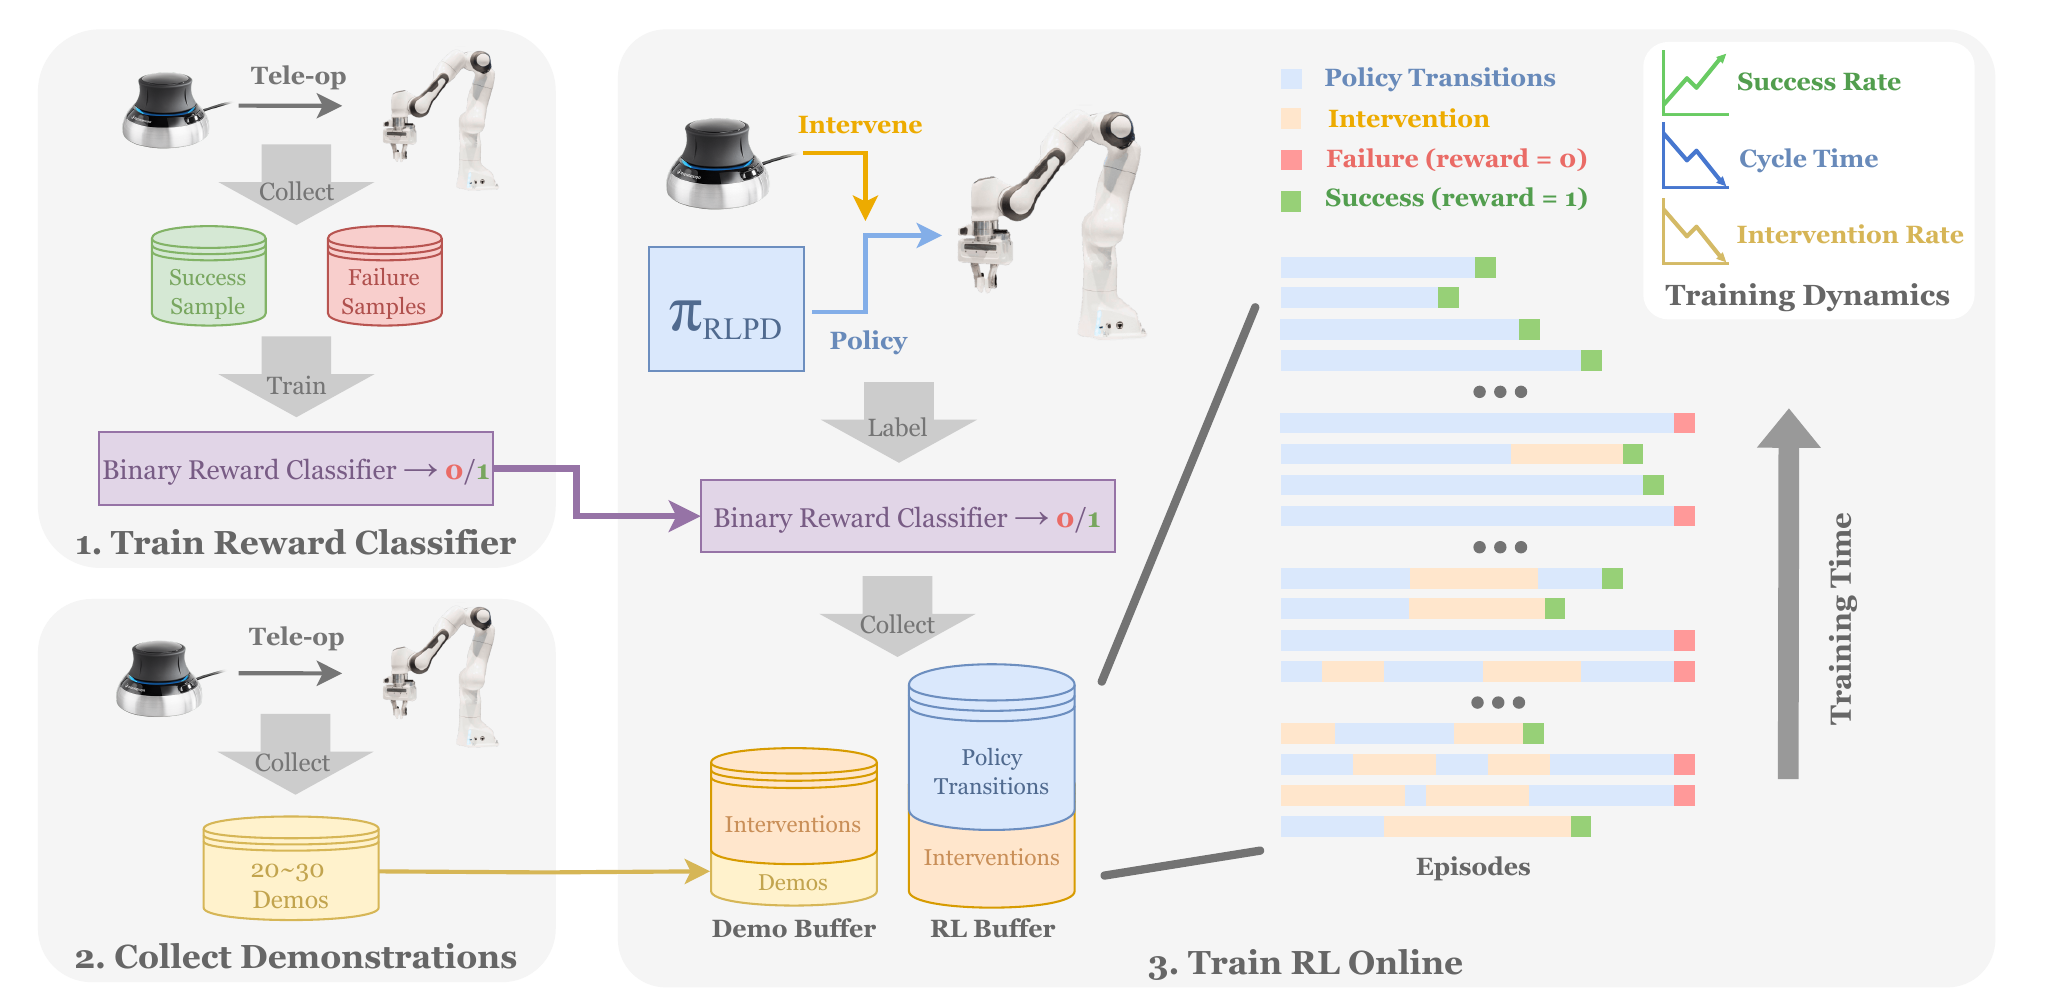
\includegraphics[width=1\linewidth,height=\textheight,keepaspectratio]{../../assets/figures/lecture16/ref/fig165-hilserl-trainproc.png}

}

\caption{HIL-SERL
训练流程：先遥操采正负样本训练奖励分类器，再采集示教装入 demo
buffer，最后在线训练并逐步减少人工干预}

\end{figure}%

左上：遥操采正负样本，训出二值奖励分类器。左下：遥操采 20 到 30 条示教进
demo
buffer。右侧：在线训练------策略与环境交互，分类器发奖励，人早期频繁干预（时间轴上黄色段多），随着策略变好干预越来越少（黄色段变稀、绿色成功标记变密）。

论文在七类真机任务上验证了这套流程，从精密插拔到动态甩锅、双臂装配都有覆盖：

\begin{figure}[H]

{\centering 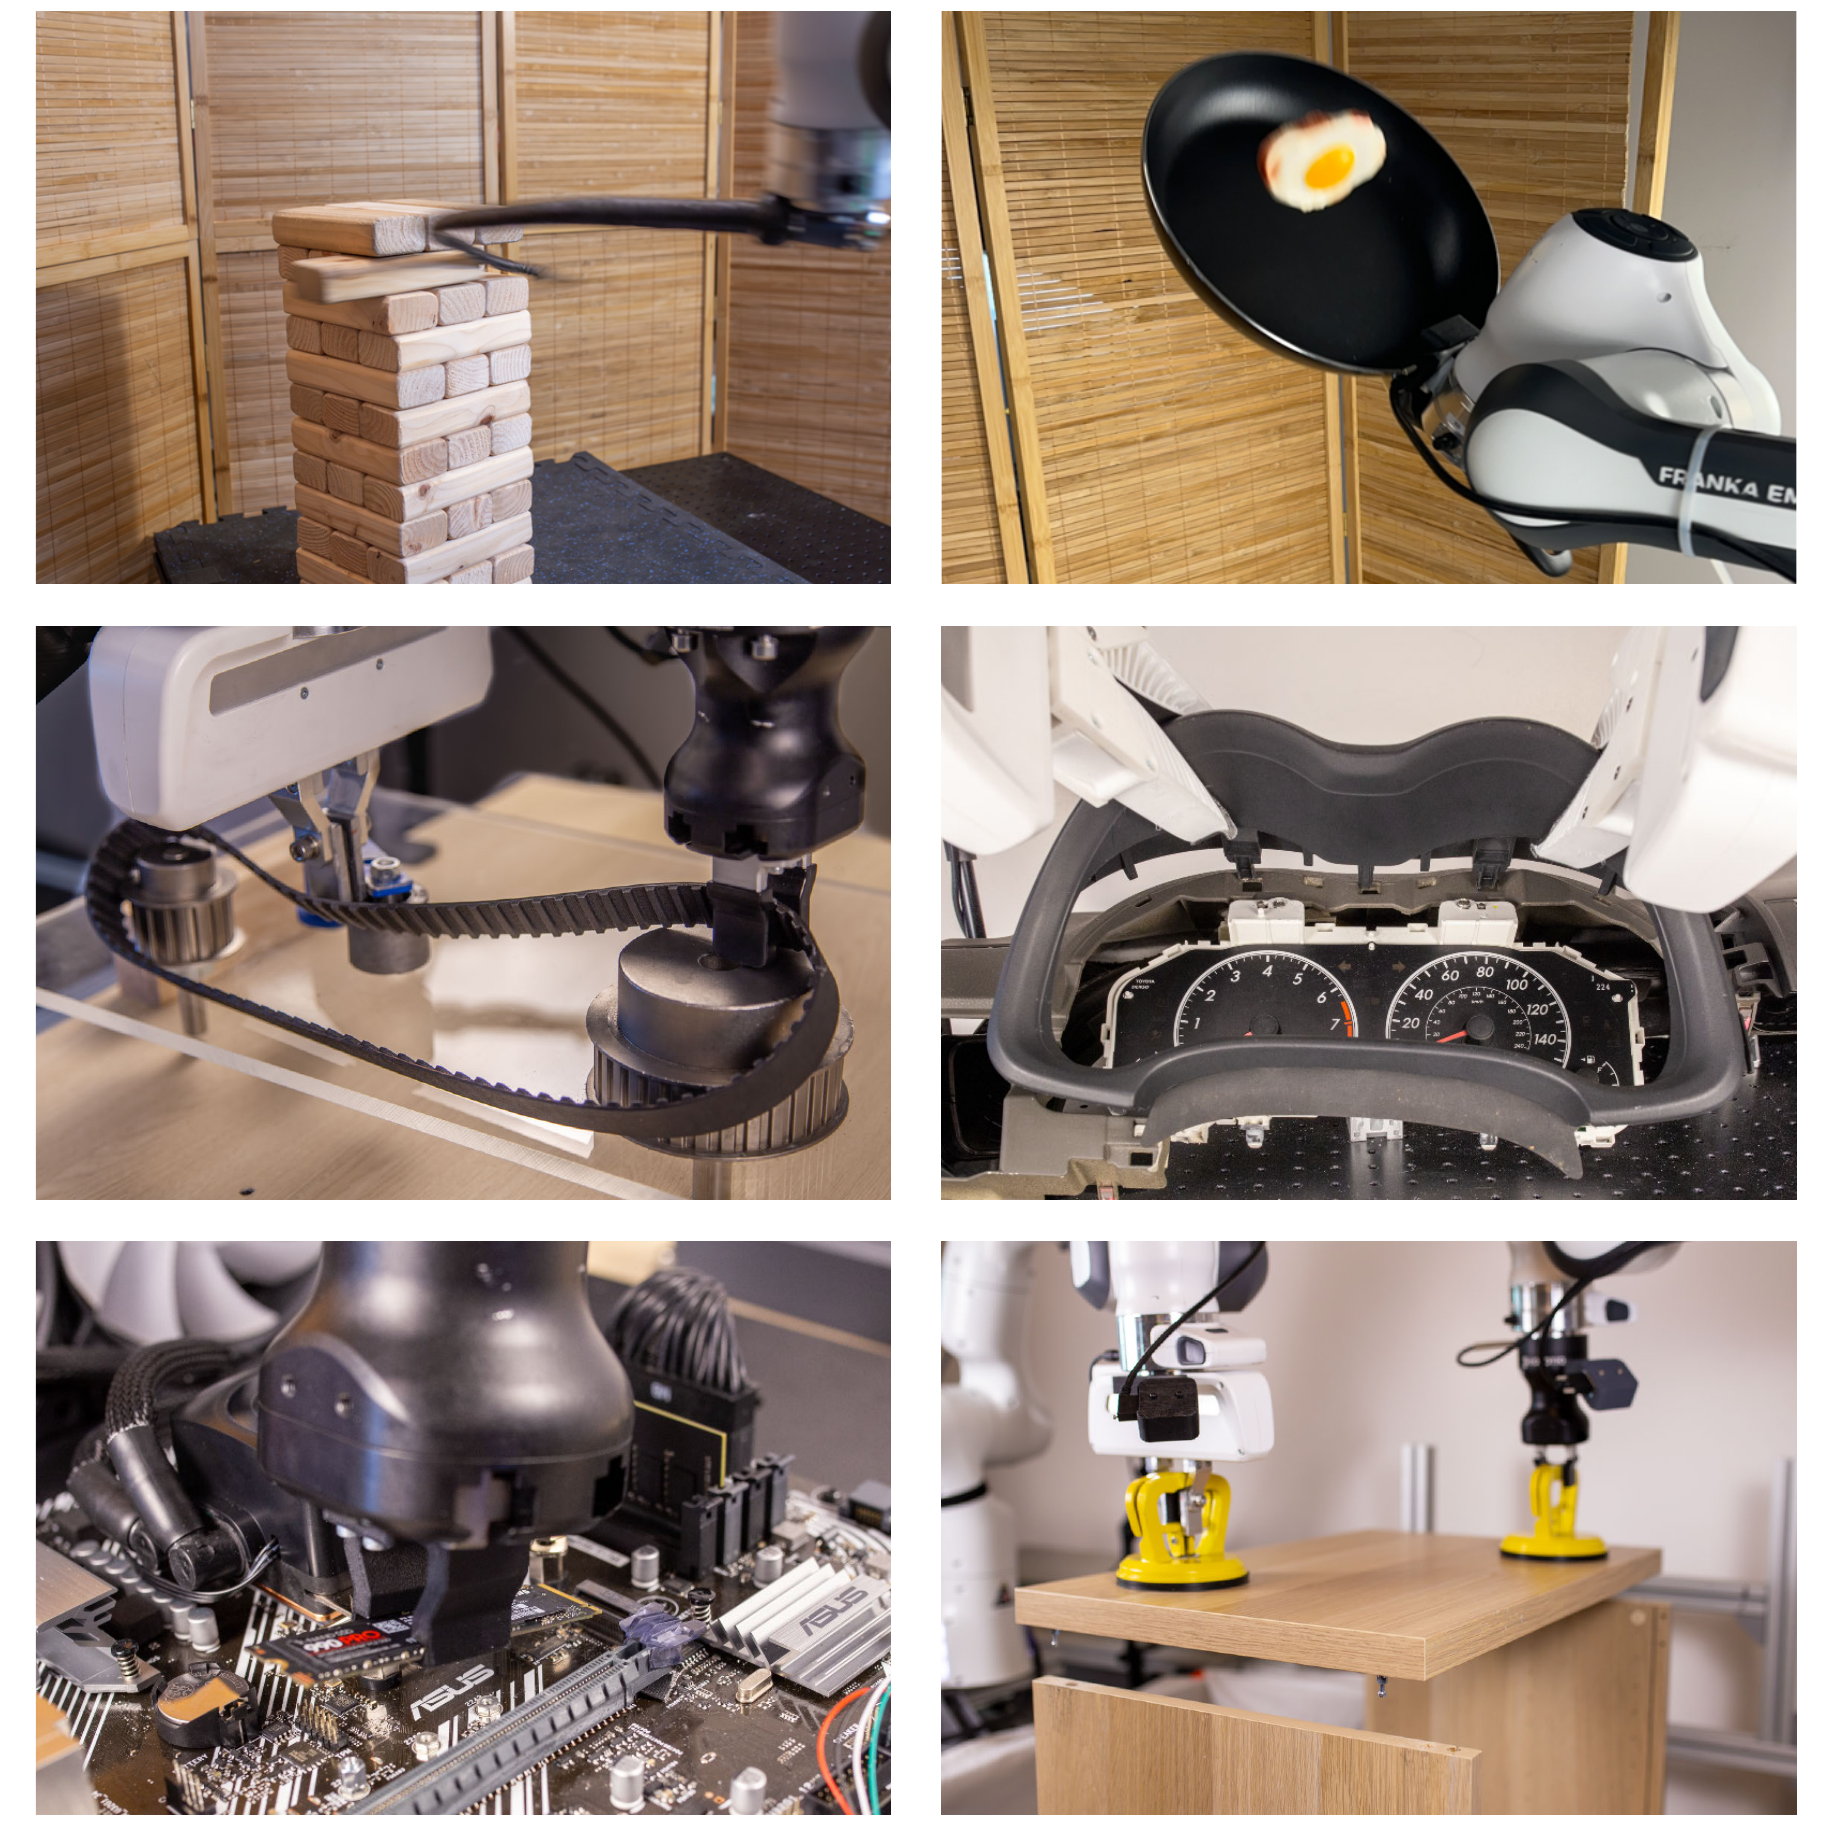
\includegraphics[width=0.88\linewidth,height=\textheight,keepaspectratio]{../../assets/figures/lecture16/ref/fig164-hilserl-tasks.png}

}

\caption{HIL-SERL
论文中的部分真机任务：抽积木、平底锅翻物、传动带装配、仪表盘装配、内存条插入、双臂搬桌板}

\end{figure}%

实验结果压成三条即可带走：

\begin{enumerate}
\def\labelenumi{\arabic{enumi}.}
\tightlist
\item
  \textbf{1 到 2 小时的真机训练}就能把多数任务练到接近 100\%
  成功率------这是''真机 RL 不可行''这个旧共识被打破的核心数字。
\item
  相对模仿学习基线，平均成功率约 \textbf{2 倍}，执行速度快约 \textbf{1.8
  倍}------RL 不只是学会了，还在按任务目标持续优化动作质量。
\item
  \textbf{干预率随训练单调下降到
  0}------人从''全程陪练''逐渐退成''旁观者''，这是系统在自我提升的最直接体征。
\end{enumerate}

\begin{figure}[H]

{\centering 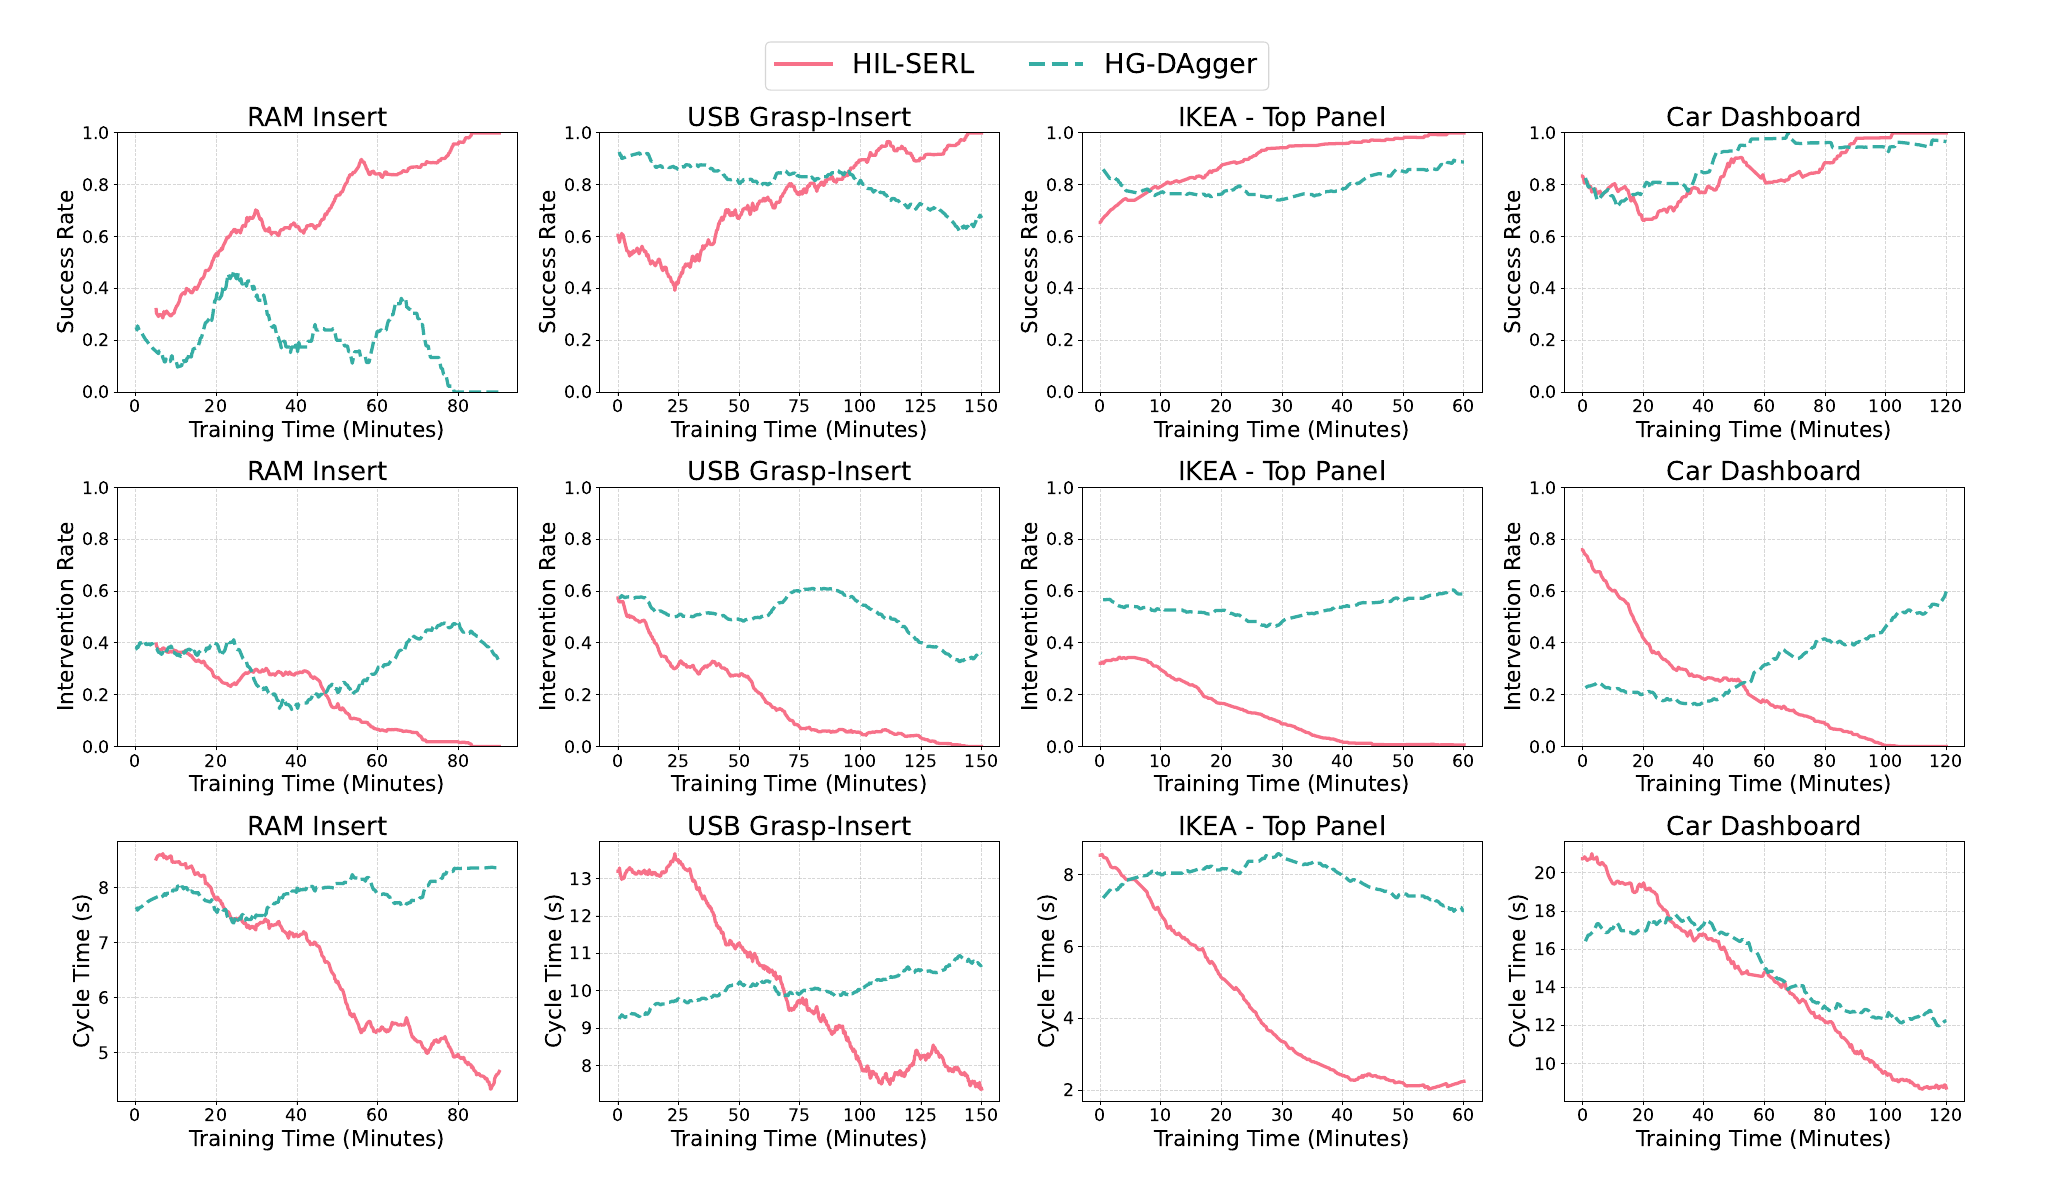
\includegraphics[width=1\linewidth,height=\textheight,keepaspectratio]{../../assets/figures/lecture16/ref/fig165-hilserl-curves.png}

}

\caption{HIL-SERL 与 HG-DAgger
在四个任务上的对照：成功率、干预率与单次执行耗时随训练时间的变化}

\end{figure}%

上图的对照值得细看：粉线（HIL-SERL）的成功率一路爬到 1.0、干预率压到
0、单次耗时持续下降；青虚线（HG-DAgger）的成功率上下震荡、干预率居高不下、耗时不见改善。同样的人力投入，监督学习''吸收''干预，强化学习''消化''干预------差距就在这。

局限性也要摊开：每个任务都要\textbf{单独}走一遍全流程（没有跨任务泛化，这正是
VLA 那条线擅长的事）；任务时长以 5 到 10
秒的短程为主；奖励分类器可能被骗。这些边界划出了它和前几讲方法的分工------本讲第
9 节会回到这张分工地图。

\subsection{8.9 没有真机：gym\_hil
仿真替代}\label{ux6ca1ux6709ux771fux673agym_hil-ux4effux771fux66ffux4ee3}

没有 SO-101 也能完整体验这套流程。LeRobot 配套的 \texttt{gym\_hil}
提供了 MuJoCo 版的 Franka Panda 抓方块环境，键盘或手柄充当干预接口：

\begin{Shaded}
\begin{Highlighting}[]
\CommentTok{\# 配置里 task 设为 PandaPickCubeKeyboard{-}v0，其余流程与真机完全一致}
\ExtensionTok{python} \AttributeTok{{-}m}\NormalTok{ lerobot.rl.actor   }\AttributeTok{{-}{-}config\_path}\NormalTok{ train\_gym\_hil\_env.json}
\ExtensionTok{python} \AttributeTok{{-}m}\NormalTok{ lerobot.rl.learner }\AttributeTok{{-}{-}config\_path}\NormalTok{ train\_gym\_hil\_env.json}
\end{Highlighting}
\end{Shaded}

采示教、起两个进程、space
接管干预------和真机同一套命令与配置结构。仿真里有物体真值，奖励可以直接判，四件套里的''奖励分类器''这一件在仿真里是可选项。建议的学习路径：先在
gym\_hil
里把全流程跑熟，再上真机------真机上每一分钟都贵，别把学工具的成本花在真机时间里。

这张有无干预的对照图说明的是另一件事------干预对\textbf{学习速度}的贡献：

\begin{figure}[H]

{\centering 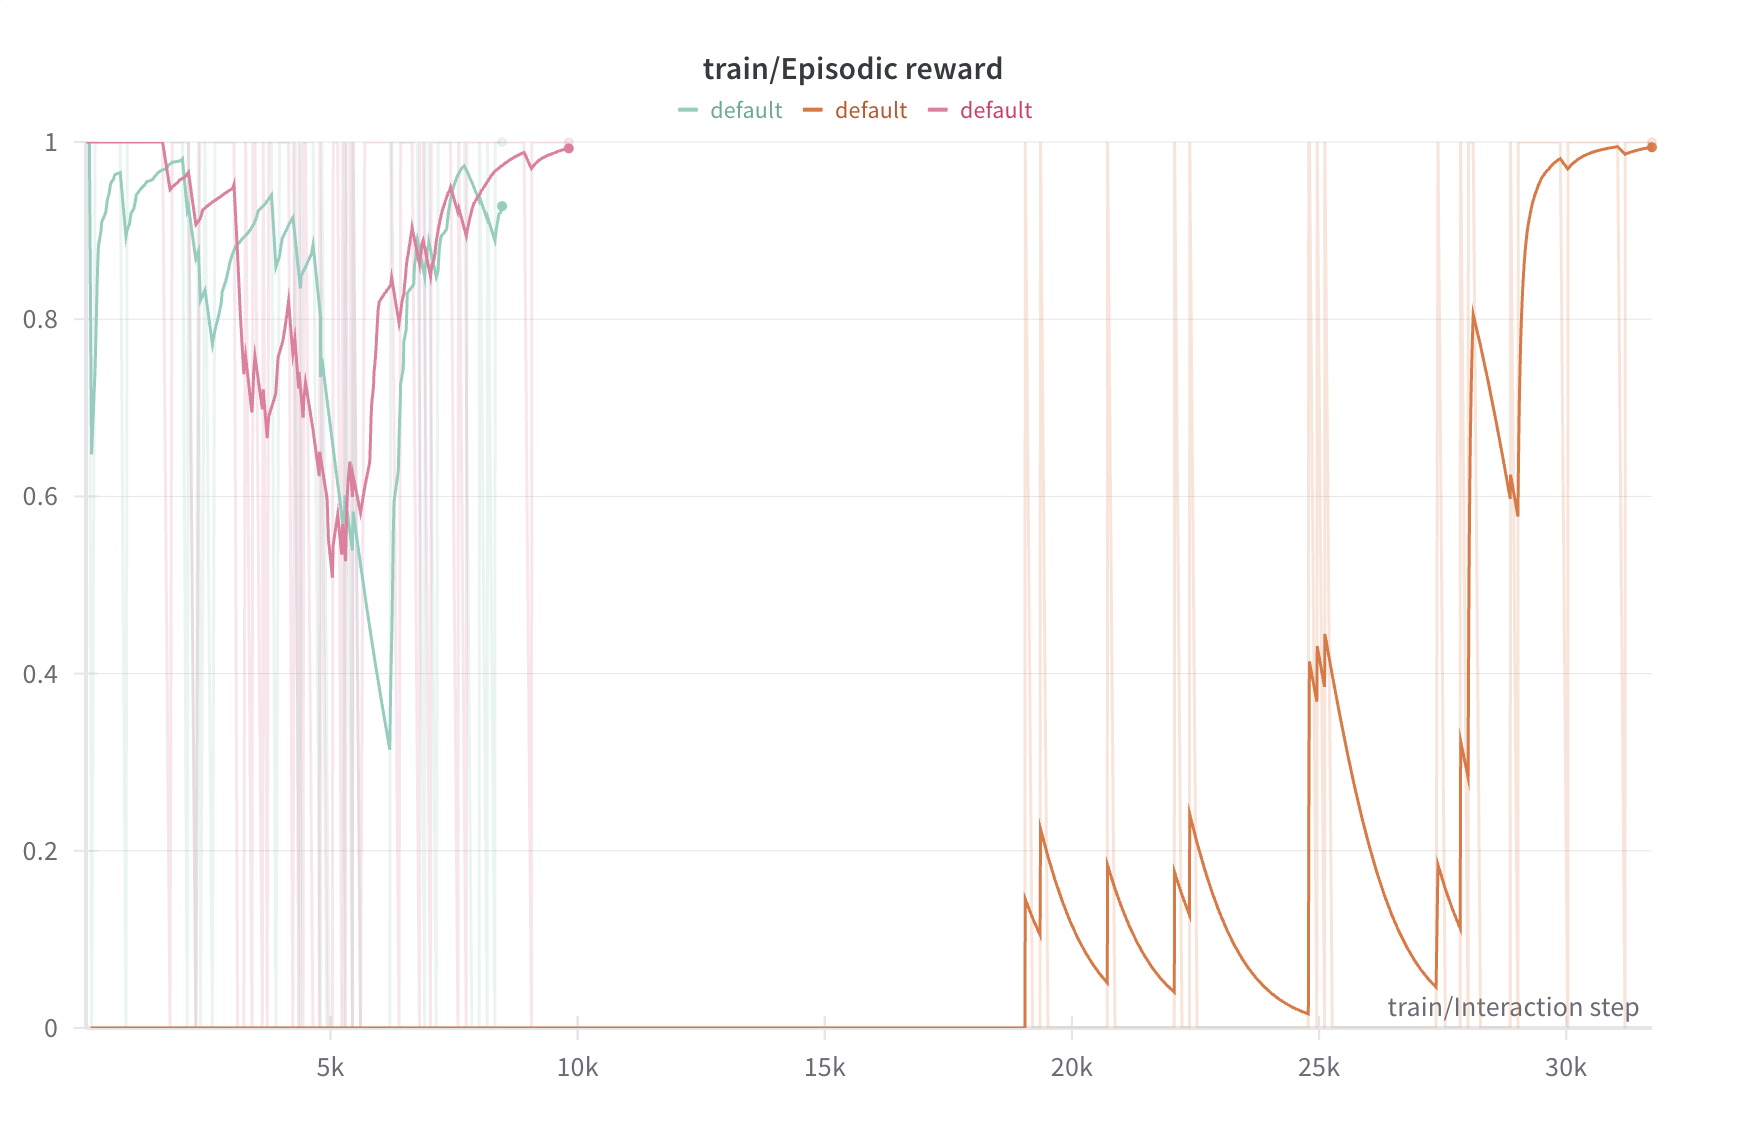
\includegraphics[width=0.78\linewidth,height=\textheight,keepaspectratio]{../../assets/figures/lecture16/ref/fig165-lerobot-hil-effect.png}

}

\caption{人工干预对学习速度的影响：无干预的训练（橙）远迟于有干预的两组（粉、蓝）达到最高回报}

\end{figure}%

橙色曲线（无干预）迟迟上不去，有人干预的两组（粉、蓝）达到最高回报所需的交互步数大幅缩短------干预不是锦上添花，而是真机
RL 能在小时级完成的关键。

\subsection{8.10
训练健康的体征：盯着干预率}\label{ux8badux7ec3ux5065ux5eb7ux7684ux4f53ux5f81ux76efux7740ux5e72ux9884ux7387}

在线训练阶段最值得盯的一张图不是回报曲线，而是\textbf{干预率曲线}。下面这张图来自
LeRobot 官方文档的抓取-提起实验。

\begin{figure}[H]

{\centering 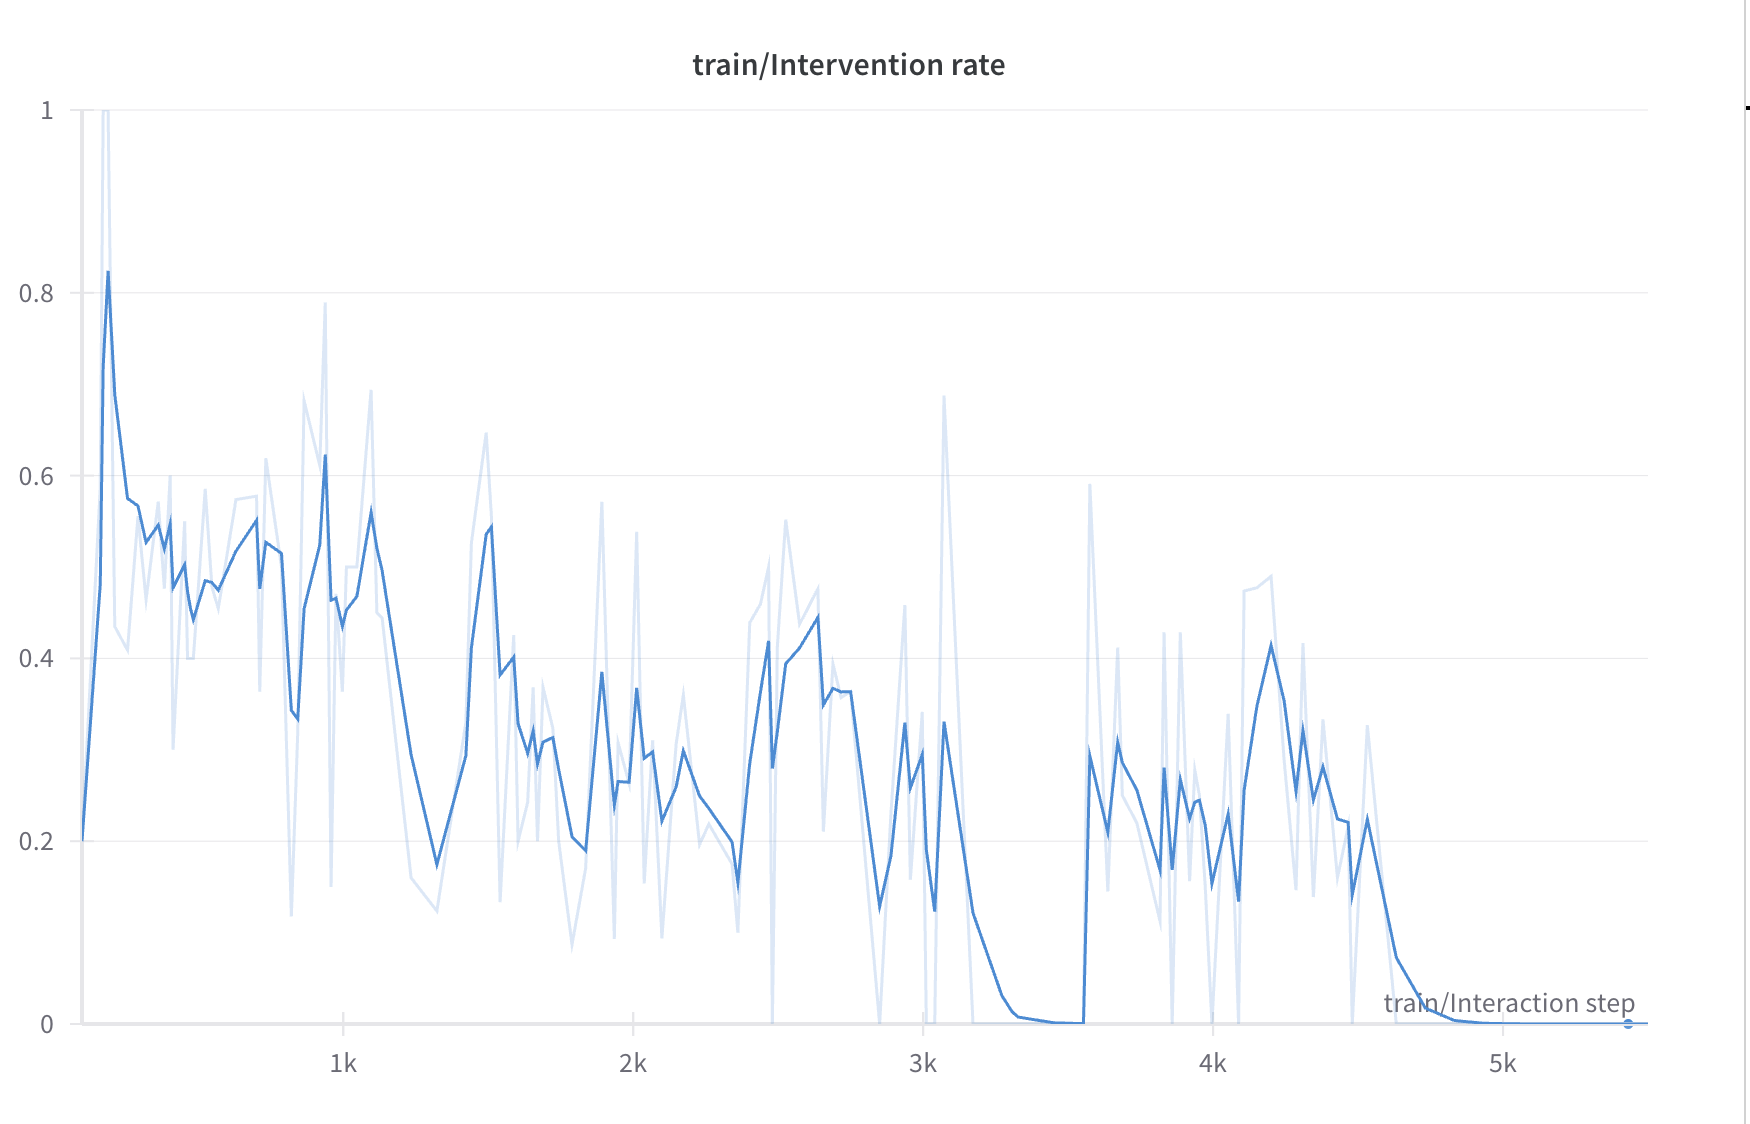
\includegraphics[width=0.78\linewidth,height=\textheight,keepaspectratio]{../../assets/figures/lecture16/ref/fig166-lerobot-intervention-rate.png}

}

\caption{一次健康训练的干预率曲线：从 0.5 上下的高位总体下行，3.3k
步附近一度归零；随后有一段回升到 0.3 左右并持续约一千步，4.7k
步后才稳定归零}

\end{figure}%

这是''健康训练''的模样：\textbf{总体趋势向下}。注意它并不单调------3.3k
步附近先归零，接着又回升到 0.3 左右拉锯了近一千步，最后才真正稳定在
0。真机训练很少给你一条干净的下降曲线；要盯的是趋势，不是某一段。如果训练半小时干预率还纹丝不动，通常说明出了问题（奖励分类器误判、边界设错、或干预方式太''代驾''），该停下来排查而不是继续耗真机时间。

本实验的 SO-101 训练前后成功率对照、干预率曲线与 rollout
视频，随课程代码仓库发布后补充。

\subsection{8.11 本节小结}\label{ux672cux8282ux5c0fux7ed3-7}

本节把 HIL-SERL 从概念一路落到我们自己的硬件上。它把''真机稀疏奖励 RL
学不动''拆成四道坎，用四件套逐一回应：示教打底解决冷启动、视觉奖励分类器解决没有上帝视角、人工干预解决探索闯祸、自动复位解决连续训练；底座是
SAC 到 RLPD 到 SERL 的 off-policy 血缘链，架构上 actor 与 learner
异步解耦保住真机的实时节拍。落到 SO-101 上，每个部件都对应 LeRobot
里的一步操作------划安全边界、采示教、框
ROI、训分类器、双进程在线训练、评测收口，每一步都是第9讲数据工具链的自然延伸；没有真机就用
gym\_hil 走完全流程。战绩：1 到 2 小时真机训练接近 100\% 成功率，约 2
倍于模仿基线；训练健康与否，第一看干预率是否持续下降。局限：单任务、短程、分类器可被骗，且真机训练全程需要人值守。它的一切素材------旧经验、示教、干预------之所以能进同一个池子，全靠
off-policy 不挑数据来源这一条根性质。

\section{9
结课全景：三种强化学习，与一条完整的链路}\label{ux7ed3ux8bfeux5168ux666fux4e09ux79cdux5f3aux5316ux5b66ux4e60ux4e0eux4e00ux6761ux5b8cux6574ux7684ux94feux8def}

\subsection{9.1 三种 RL
形态对照}\label{ux4e09ux79cd-rl-ux5f62ux6001ux5bf9ux7167}

课程的强化学习三部曲到此收官。三讲各用了一种形态的
RL，放进一张表里，差异一目了然：

\begin{center}
\begin{tabular}{@{}>{\raggedright\arraybackslash}p{\dimexpr 0.1336\linewidth - 2\tabcolsep\relax} >{\raggedright\arraybackslash}p{\dimexpr 0.2905\linewidth - 2\tabcolsep\relax} >{\raggedright\arraybackslash}p{\dimexpr 0.2203\linewidth - 2\tabcolsep\relax} >{\raggedright\arraybackslash}p{\dimexpr 0.3555\linewidth - 2\tabcolsep\relax}@{}}
\toprule\noalign{}
 & 第14讲 & 第15讲 & 第16讲 \\
\midrule\noalign{}
载体 & G1 人形行走/动作跟随 & VLM 数数、VLA-0 操作 & SO-101 接触任务 \\
训练地点 & 仿真（大规模并行） & 仿真 rollout / GPU 答题 & \textbf{真机在线} \\
动作 & 连续关节控制 & 离散 token & 连续 EE 控制 \\
奖励 & 手写密集奖励 & 可验证规则，稀疏但免费 & \textbf{学出来的}视觉 0/1 \\
数据方式 & on-policy & on-policy & \textbf{off-policy} \\
critic & 有（GAE 基线） & 无（组内相对优势） & 有（Q 函数，主角） \\
人的角色 & 写奖励函数 & 写判分规则 & \textbf{示教 + 在线干预} \\
代表算法 & PPO & GRPO & SAC（RLPD/HIL-SERL） \\
本讲演示阶梯 & REINFORCE→A2C→PPO & 单一 GRPO & 表格Q→DQN→DDPG→TD3→SAC→squint（六级 off-policy） \\
\bottomrule\noalign{}
\end{tabular}
\end{center}

这张表也是一张\textbf{选型地图}：有仿真、能并行、奖励好写------on-policy
大力出奇迹（第14讲）；策略本体是生成模型、结果可规则验证------GRPO
后训练（第15讲）；必须在真机上学、样本以秒计费------off-policy
加人在环（本讲）。三种形态没有高下，只有场景匹配。

\subsection{9.2
从第8讲到第16讲：一条链路}\label{ux4eceux7b2c8ux8bb2ux5230ux7b2c16ux8bb2ux4e00ux6761ux94feux8def}

把镜头拉远，这九讲其实只讲了一件事------\textbf{一台机器人怎么从零获得并持续改进一个技能}：

\begin{itemize}
\tightlist
\item
  \textbf{第8讲}立了骨架：端到端 policy，观测进、动作出，rollout
  才是唯一的裁判。
\item
  \textbf{第9讲}解决原料：遥操作采集、LeRobot
  数据闭环------今天它的主从臂和数据格式在 RL 里原样复用。
\item
  \textbf{第10讲}给了第一批可用的大脑：ACT、Diffusion Policy、Flow
  Matching，模仿学习把示教''学得像''。
\item
  \textbf{第11到13讲}把大脑换成通才：VLA
  家族------预训练带来语言理解与跨任务泛化，微调把它对齐到你的机器人。
\item
  \textbf{第14讲}引入第二种学习范式：不再模仿，而是试错------策略梯度到
  PPO，在仿真里大规模练。
\item
  \textbf{第15讲}把两条线接起来：RL 作为后训练外环，让模仿学出来的 VLA
  自我提升。
\item
  \textbf{本讲}走完最后一公里：off-policy
  加人在环，让学习直接发生在真机上------模仿给底子，人保驾，RL
  超越示范者。而且这条 RL 线还会反哺 VLA：SO-101
  阶梯顶端那个从像素学会的视觉策略，顺手 rollout
  又换外观重渲，就生成出第9讲与第12讲用来微调 VLA 的那批仿真数据集（第 6
  节）------``RL 生成数据 → VLA 微调''的仿真数据闭环就此合上。
\end{itemize}

模仿学习与强化学习在这条链路上不是对手而是接力：\textbf{示教决定起点，试错决定上限，真机决定成色}。课程后续将继续走向世界模型等更前沿的方向，而无论模型形态怎么变，这条''数据-策略-改进''的闭环都是底层不变的骨架。

\section{10 本讲小结}\label{ux672cux8bb2ux5c0fux7ed3}

\subsection{10.1 主线回顾}\label{ux4e3bux7ebfux56deux987e}

这一讲从一笔账出发：真机上样本贵三个数量级，on-policy''采完即弃''的奢侈打法玩不起，于是换
off-policy------行为策略与目标策略解耦，旧经验、示教、干预统统进 replay
buffer 反复用；数学根基是贝尔曼等式不挑数据来源。我们先在 CartPole 上把
Q 函数、经验回放、目标网络跑成代码，从手工分桶的表格 Q 走到吃原始状态的
DQN。随后在 SO-101 的 ReachCube 上从零爬了一条 off-policy 阶梯：DDPG
用确定性 Actor 把 off-policy 带进连续动作（过程中诊断了观测不归一化把
\texttt{tanh} 顶进饱和、Actor 梯度冻结的典型坑），TD3 用双 Critic
取小治好高估、却仍卡在探索，SAC 把最大熵写进训练目标、成功率一举从 0
冲到 0.99，squint 再把输入换成像素、Critic 换成 C51 分布式，从 16
像素学会并顺手生成出 VLA 微调数据。接着回到 G1
行走验证规模化：FastSAC/FastTD3 单卡 15 分钟练成能上真机的行走。最后
HIL-SERL 把 off-policy
带上真机------示教打底、视觉分类器发奖、人在环纠偏、自动复位撑连续训练，1
到 2 小时把接触型任务练到接近 100\%，落到 SO-101 上就是一整套 LeRobot
工作流，干预率下降就是训练健康的体征。

\subsection{10.2 方法演进链}\label{ux65b9ux6cd5ux6f14ux8fdbux94fe}

这一讲织了两条演进链。一条是\textbf{算法阶梯}，每一级只补上一级的一个短板：

\[\text{表格 Q} \;\to\; \text{DQN} \;\to\; \text{DDPG} \;\to\; \text{TD3} \;\to\; \text{SAC} \;\to\; \text{squint}\]

分桶到函数近似、离散到连续、单 Critic 到双
Critic、外加噪声到最大熵、标量到分布式视觉------一步一个知识点。另一条是把
SAC 带上真机的\textbf{工程血缘链}：

\[\text{SAC} \;\to\; \text{RLPD} \;\to\; \text{SERL} \;\to\; \text{HIL-SERL}\]

能力、样本效率、工程骨架、真机落地------每一步只加一块砖。旁支上，FastTD3/FastSAC
证明同一套 off-policy 底座在大规模并行仿真里同样占优。

\begin{quote}
一句话总结：真机上的强化学习是一门''省''的艺术------off-policy
把每条经验用到极致，人在环把每次失败挡在损失之外，从 CartPole 一路爬到
squint 再到
HIL-SERL，讲的都是同一件事：用最少的真机样本，把一个接触型技能在 1 到 2
小时内学出来。
\end{quote}

\section{参考资料}\label{ux53c2ux8003ux8d44ux6599}

{[}1{]} HAARNOJA T, ZHOU A, ABBEEL P, et al.~Soft actor-critic:
Off-policy maximum entropy deep reinforcement learning with a stochastic
actor{[}EB/OL{]}. (2018-01-04). https://arxiv.org/abs/1801.01290.

{[}2{]} FUJIMOTO S, VAN HOOF H, MEGER D. Addressing function
approximation error in actor-critic methods{[}EB/OL{]}. (2018-02-26).
https://arxiv.org/abs/1802.09477.

{[}3{]} SEO Y, SFERRAZZA C, GENG H, et al.~FastTD3: Simple, fast, and
capable reinforcement learning for humanoid control{[}EB/OL{]}.
(2025-05-28). https://arxiv.org/abs/2505.22642.

{[}4{]} SEO Y, SFERRAZZA C, CHEN J, et al.~Learning sim-to-real humanoid
locomotion in 15 minutes{[}EB/OL{]}. (2025-12-01).
https://arxiv.org/abs/2512.01996.

{[}5{]} LUO J, XU C, WU J, et al.~Precise and dexterous robotic
manipulation via human-in-the-loop reinforcement learning{[}EB/OL{]}.
(2024-10-29). https://arxiv.org/abs/2410.21845.

{[}6{]} BALL P J, SMITH L, KOSTRIKOV I, et al.~Efficient online
reinforcement learning with offline data{[}EB/OL{]}. (2023-02-06).
https://arxiv.org/abs/2302.02948.

{[}7{]} LUO J, HU Z, XU C, et al.~SERL: A software suite for
sample-efficient robotic reinforcement learning{[}EB/OL{]}.
(2024-01-29). https://arxiv.org/abs/2401.16013.

{[}8{]} KELLY M, SIDRANE C, DRIGGS-CAMPBELL K, et al.~HG-DAgger:
Interactive imitation learning with human experts{[}EB/OL{]}.
(2018-10-05). https://arxiv.org/abs/1810.02890.

{[}9{]} CADENE R, ALIBERT S, SOARE S, et al.~LeRobot: State-of-the-art
machine learning for real-world robotics in PyTorch{[}EB/OL{]}.
https://github.com/huggingface/lerobot.

{[}10{]} SIMONINI T, SANSEVIERO O. The Hugging Face deep reinforcement
learning course{[}EB/OL{]}. (2023){[}2026-07-04{]}.
https://huggingface.co/learn/deep-rl-course.




\end{document}
